% -*- latex -*-

%\documentclass[journal]{vgtc}                % final (journal style)
\documentclass[review,journal]{vgtc}         % review (journal style)
%\documentclass[widereview]{vgtc}             % wide-spaced review
%\documentclass[preprint,journal]{vgtc}       % preprint (journal style)
%\documentclass[electronic,journal]{vgtc}     % electronic version, journal

%% Uncomment one of the lines above depending on where your paper is
%% in the conference process. ``review'' and ``widereview'' are for review
%% submission, ``preprint'' is for pre-publication, and the final version
%% doesn't use a specific qualifier. Further, ``electronic'' includes
%% hyperreferences for more convenient online viewing.

%% Please use one of the ``review'' options in combination with the
%% assigned online id (see below) ONLY if your paper uses a double blind
%% review process. Some conferences, like IEEE Vis and InfoVis, have NOT
%% in the past.

%% Please note that the use of figures is not permitted on the first page
%% of the journal version.  Figures should begin on the second page and be
%% in CMYK or Grey scale format, otherwise, colour shifting may occur
%% during the printing process.  Papers submitted with figures on the
%% first page will be refused.

%% These three lines bring in essential packages: ``mathptmx'' for Type 1
%% typefaces, ``graphicx'' for inclusion of EPS figures. and ``times''
%% for proper handling of the times font family.

\usepackage{mathptmx}
\usepackage{graphicx}
\usepackage{times}

%% We encourage the use of mathptmx for consistent usage of times font
%% throughout the proceedings. However, if you encounter conflicts
%% with other math-related packages, you may want to disable it.

%% If you are submitting a paper to a conference for review with a double
%% blind reviewing process, please replace the value ``0'' below with your
%% OnlineID. Otherwise, you may safely leave it at ``0''.
\onlineid{vis-1146}

%% declare the category of your paper, only shown in review mode
\vgtccategory{Research}

%% allow for this line if you want the electronic option to work properly
\vgtcinsertpkg

%% In preprint mode you may define your own headline.
%\preprinttext{To appear in an IEEE VGTC sponsored conference.}

\usepackage{amsfonts}
\usepackage{amssymb}
\usepackage{amsmath}
\usepackage{graphicx}
\usepackage{varioref}
\usepackage{fancyvrb}
%\usepackage{cite}
\usepackage{subfigure}
\usepackage{xspace}
\usepackage{clrscode}
\usepackage[pdfstartview=FitH]{hyperref}

\title{Diverging Color Maps for Scientific Visualization}


%% This is how authors are specified in the journal style

%% %% indicate IEEE Member or Student Member in form indicated below
%% \author{Roy G. Biv, Ed Grimley, \textit{Member, IEEE}, and Martha Stewart}
%% \authorfooter{
%% %% insert punctuation at end of each item
%% \item
%%   Roy G. Biv is with Starbucks Research, E-mail: roy.g.biv@aol.com.
%% \item
%%   Ed Grimley is with Grimley Widgets, Inc., E-mail: ed.grimley@aol.com.
%% \item
%%   Martha Stewart is with Martha Stewart Enterprises at Microsoft
%%   Research, E-mail: martha.stewart@marthastewart.com.
%% }

\author{Kenneth~Moreland, \textit{Member, IEEE}}
\authorfooter{
\item
  Kenneth Moreland is with Sandia National Laboratories, E-mail: kmorel@sandia.gov
}

\shortauthortitle{Moreland: Diverging Color Maps for Scientific
  Visualization}

%% Abstract section
\abstract{One of the most fundamental features of scientific visualization
  is the process of mapping scalar values to colors.  This process allows
  us to view scalar fields by coloring surfaces and volumes.
  Unfortunately, the majority of scientific visualization tools and
  research are still using a color map that is famous for its
  ineffectiveness: the rainbow color map.  This color map, which
  na\"{i}vely sweeps through the most saturated colors that a display can
  reproduce in rainbow color order, is well known for its ability to
  obscure data, introduce artifacts, and confuse users.

  Although many alternate color maps have been proposed, none have achieved
  widespread adoption by the visualization community for scientific
  visualization.  In this paper, I explore the use of diverging color maps
  (sometimes also called ratio, bipolar, or double-ended color maps) for
  use in scientific visualization.  I provide a diverging color map that
  generally performs well in scientific visualization applications and that
  is a clear replacement for the rainbow color map.  I also present an
  algorithm that allows users to easily generate their own customized color
  maps.  I hope, once and for all, we can kill the use of the rainbow color
  map for serious scientific visualization applications.
} % End of abstract

%% Keywords that describe your work.
\keywords{color, scientific visualization}

%% ACM Computing Classification System (CCS). 
%% See <http://www.acm.org/class/1998/> for details.
%% The ``\CCScat'' command takes four arguments.

\CCScatlist{ % not used in journal version
  \CCScat{I.3.m}{Computing Methodologies}{Computer Graphics}{Miscellaneous};
  \CCScat{H.5.2}{Information Interfaces and Presentation}%
    {User Interfaces}{Screen design};
  \CCScat{H.1.2}{Models and Principles}{User/Machine Systems}{Human factors}
}

% Make fonts slightly bigger for equations to make them easier to read.
\DeclareMathSizes{9}{9}{7}{6}

% Commands I use for citing.
\newcommand{\lcite}[1]{~\cite{#1}}
\newcommand{\scite}[1]{~\cite{#1}}

% Put figures inline with text when possible
\usepackage{float}
\floatplacement{figure}{htb}

% Avoid putting figures on their own page.
\renewcommand{\textfraction}{0.05}
\renewcommand{\topfraction}{0.95}
\renewcommand{\dbltopfraction}{0.95}

% Make sure this is big enough so that only big figures end up on their own
% page but small enough so that if a figure does have to be on its own
% page, it won't push everything to the bottom because it's not big enough
% to have its own page.
\renewcommand{\floatpagefraction}{.75}
\renewcommand{\dblfloatpagefraction}{.75}

\newcommand{\sticky}[1]{\textsc{[#1]}}

\newcommand{\RGB}{RGB\xspace}
\newcommand{\CMYK}{CMYK\xspace}
\newcommand{\XYZ}{XYZ\xspace}
\newcommand{\Lab}{CIELAB\xspace}
\newcommand{\Luv}{CIELUV\xspace}
\newcommand{\Msh}{Msh\xspace}
\newcommand{\DeltaE}{\ensuremath{\Delta{}E}\xspace}
\newcommand*{\cvec}[1]{\mathbf{#1}}


\begin{document}

%% The ``\maketitle'' command must be the first command after the
%% ``\begin{document}'' command. It prepares and prints the title block.

%% the only exception to this rule is the \firstsection command
\firstsection{Introduction}
\label{sec:Introduction}

\maketitle

At its core, visualization is the process of providing a visual
representation of data.  One of the most fundamental and important aspects
of this process is the mapping of numbers to colors.  This mapping allows
us to pseudocolor an image or object based on varying numerical data.
Obviously, the choice of color map is important to allow the viewer to
easily perform the reverse mapping back to scalar values.

\begin{figure}
  \centering
  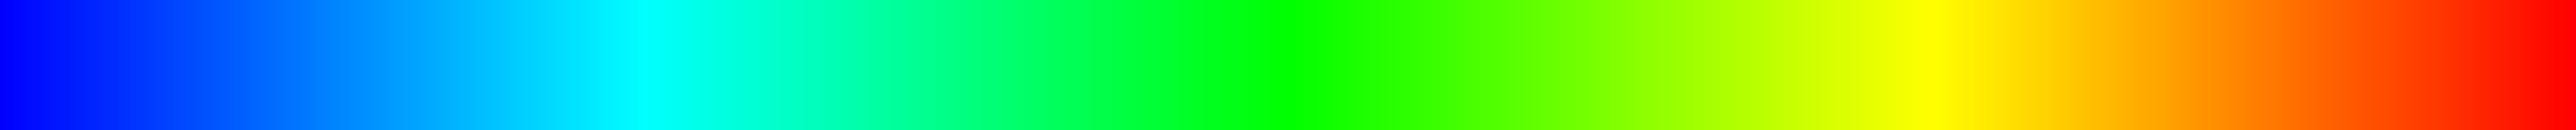
\includegraphics[width=2.5in]{images/RainbowBar}
  \caption{The rainbow color map.  Know thy enemy.}
  \label{fig:RainbowColorMap}
\end{figure}

By far, the most common color map used in scientific visualization is the
rainbow color map, shown in Figure~\ref{fig:RainbowColorMap}.  In a recent
review on the use of color maps, Borland and Taylor\scite{Borland07} find
that the rainbow color map was used as the default in 8 out of the 9
toolkits they examined.  Borland and Taylor also find that in IEEE
Visualization papers from 2001 to 2005 the rainbow color map is used 51
percent of the time.

Despite its popularity, the rainbow color map has been shown to be a poor
choice for a color map in nearly all problem domains.  This well-studied
field of perception shows that the rainbow color map obfuscates, rather
than clarifies, the display of data in a variety of ways\lcite{Borland07}.
The choice of a color map can be a complicated decision that depends on the
visualization type and problem domain, but the rainbow color map is a poor
choice for almost all of them.

Why are so many visualization scientists and developers, experts who
should know better, still using the rainbow color map?
There are many contributing factors, two of which are clearly significant.
First is the ease with which rainbow color maps
can be created.  I was guilty of creating rainbow color maps
long before learning anything about color spaces and human perception.  It
was my first choice and I was pleased with the colorful images, ignorant of
their dubious scientific value.

A second major contributor to the dominance of the rainbow color map is the
lack of a clear alternative, especially in terms of scientific
visualization.  There are many publications that recommend
very good choices for color maps\lcite{Brewer05,Levkowitz92,Rheingans99,Ware04}.
However, each candidate has its features and flaws, and the choice of
the ``right'' one is difficult.  The conclusion of
all these publications is to pick from a variety of color maps for the best
choice for a domain-specific visualization.  Although this is reasonable
for the designer of a targeted visualization application, a general
purpose application, designed for multiple problem domains, would have to
push this decision to the end-user with a dizzying array of color map
choices.  In our experience the user, who seldom has the technical
background to make an informed decision, usually chooses a rainbow color map.

This paper recommends a good default
color map for general purpose scientific visualization.  The
color map derived here is an all-around good performer: it works well for
low and high frequency data, orders the data, is perceptually linear,
behaves well for observers with color-deficient vision, and has reasonably
low impact on the shading of three-dimensional surfaces.


\section{Previous Work}
\label{sec:PreviousWork}

This previous work section is divided into two parts.  First is a
quick review on previously proposed color maps that lists the pros and
cons of each.  Second is a quick review on color spaces,
which is relied upon in subsequent discussions.

\subsection{Color Maps}
\label{sec:PreviousWork:ColorMaps}

The rainbow color map is an
extremely poor choice.  Based on the colors of light at different
wavelengths, the rainbow color map's design has nothing to do with how
humans perceive color.  This results in multiple problems when humans try
to do the reverse mapping from colors back to numbers.

The first problem is that the colors do not follow any natural perceived
ordering.  Perceptual experiments show that although a test subject with no
prior training will always order grayscale colors in order of luminance (in
one direction or the other), the test subjects will order rainbow colors in
numerous different ways\lcite{Ware04}.

The second problem is that the perceptual changes in the colors are not
uniform.  The colors appear to change faster in the cyan and yellow
regions, which can cause Mach bands in those regions.  The colors appear to
change more slowly in the blue, green, and red regions, which creates larger
bands of color.  These bands can hide important changes in the
underlying data.  Thus, nonuniform perceptual changes
simultaneously introduce artifacts and obfuscate real
data\lcite{Borland07} as demonstrated in
Figure~\ref{fig:RainbowSpatialContrast}.

\begin{figure}
  \centering
  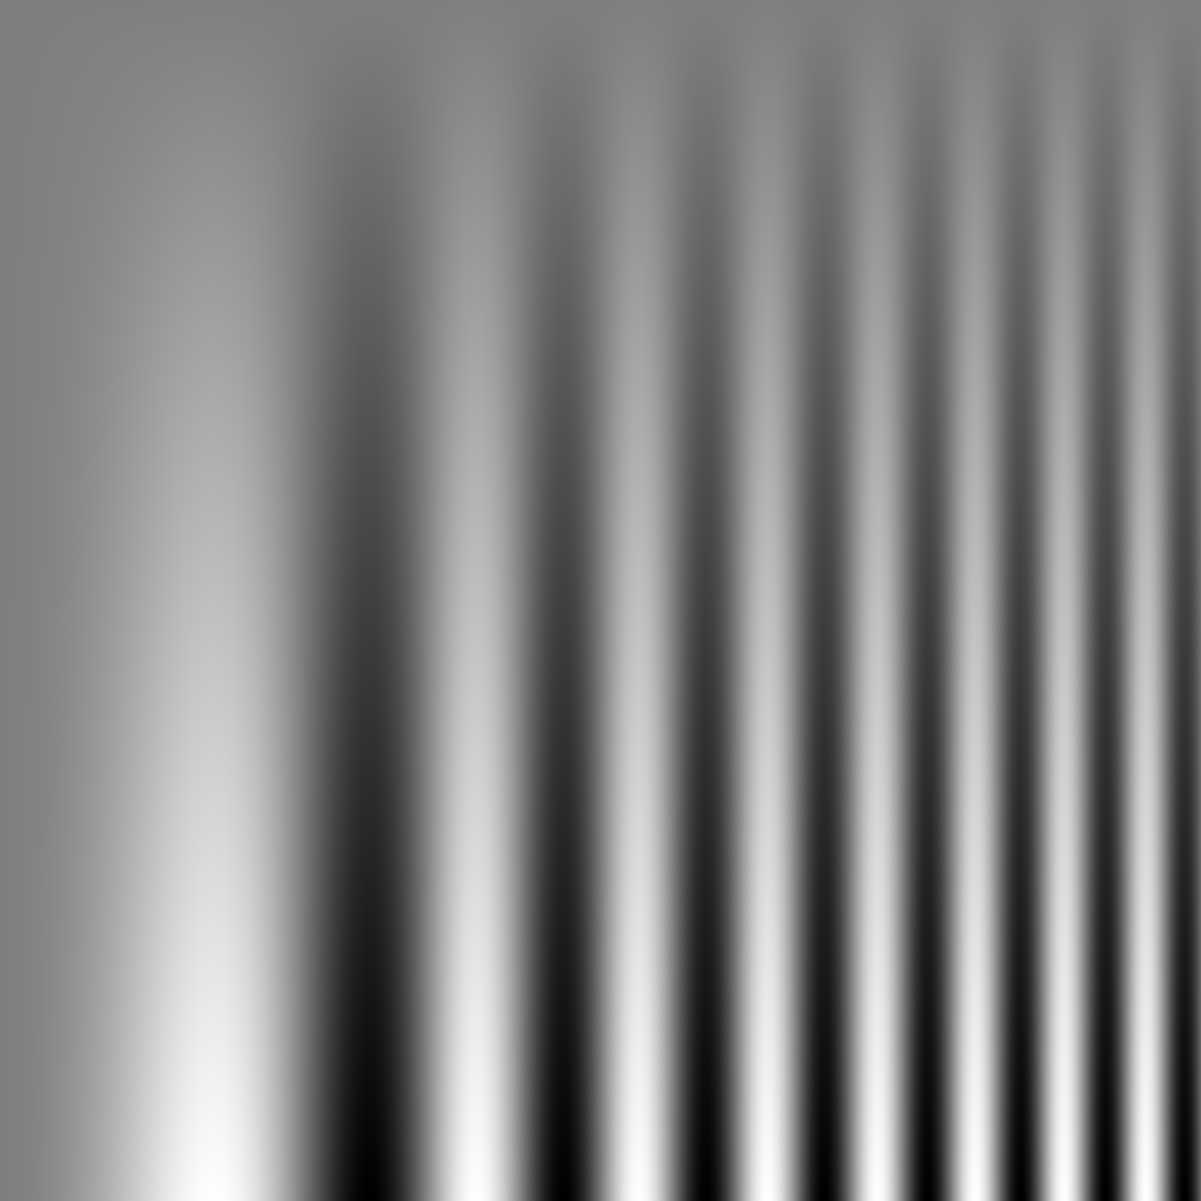
\includegraphics[width=1.0in]{images/GrayscaleSpatialContrast}
  \qquad
  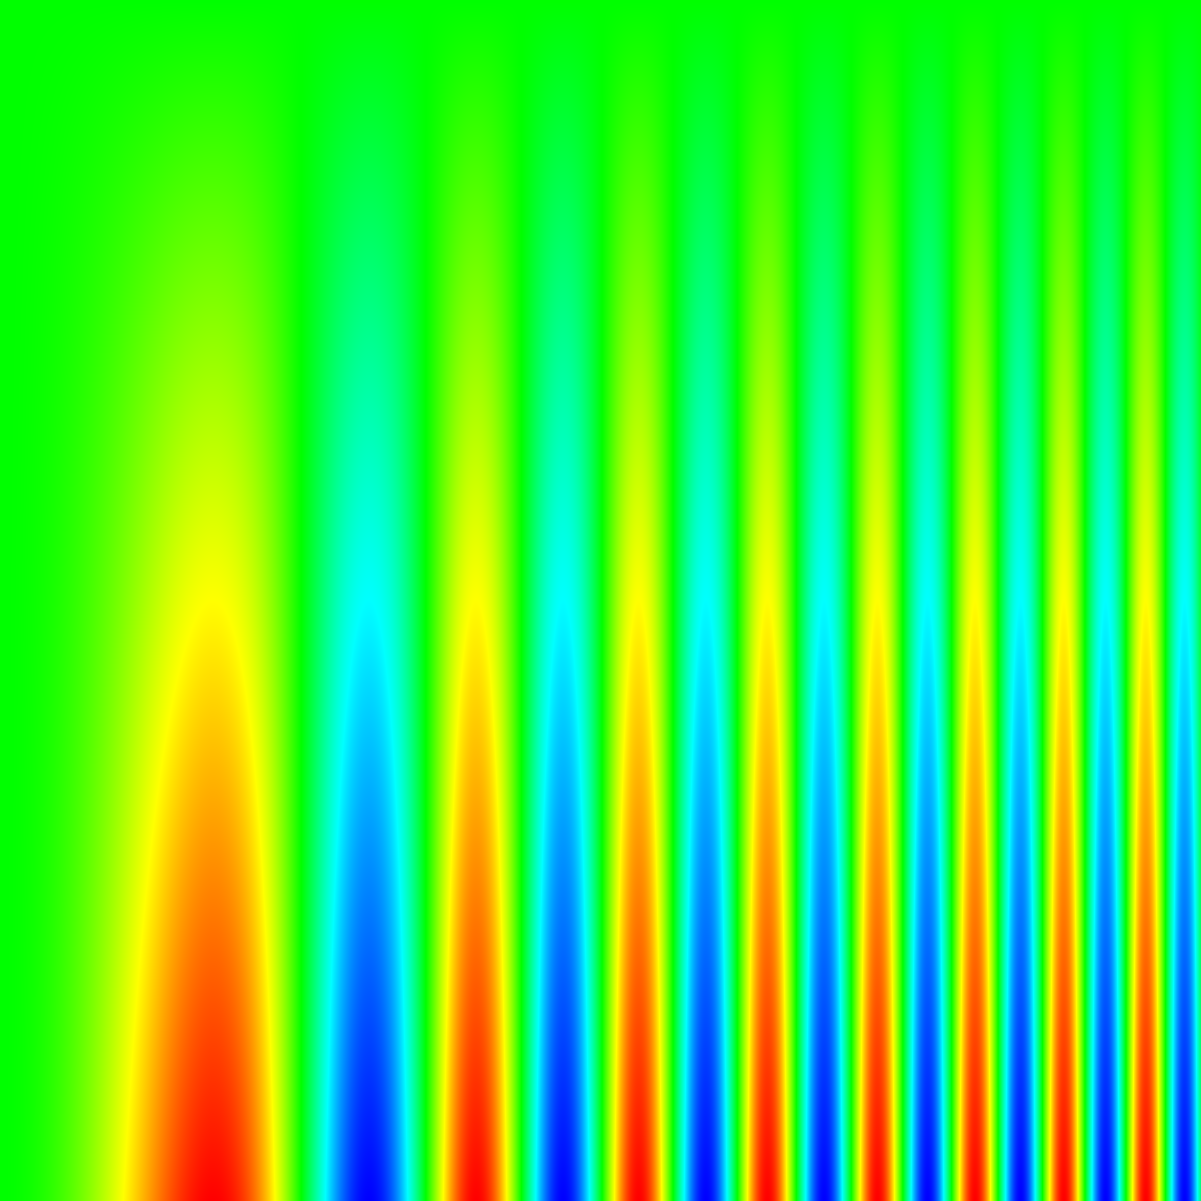
\includegraphics[width=1.0in]{images/RainbowSpatialContrast}
  \caption{A spatial contrast sensitivity function.  The frequency of the
    function increases from left to right, and the contrast increases from
    top to bottom.  Notice that the grayscale mapping (on the left)
    faithfully reproduces the function.  The rainbow color mapping (on the
    right) hides the variation in the low contrast region and appears less
    smooth in the high-contrast, low-frequency region.}
  \label{fig:RainbowSpatialContrast}
\end{figure}

A third problem with the rainbow color map is that it is sensitive to
deficiencies in vision.  Roughly 5\% of the population cannot distinguish
between the red and green colors.  These unfortunate souls cannot
distinguish many colors considered ``far apart'' in the rainbow color
map\lcite{Light04}.

\begin{figure}
  \centering
  
\includegraphics[width=2.5in]{images/GrayscaleBar}
  \caption{The grayscale color map.}
  \label{fig:GrayscaleColorMap}
\end{figure}
Better color maps exist.  A very simple one is the grayscale
color map shown in Figure~\ref{fig:GrayscaleColorMap}.  Completely devoid
of any chromaticity, this map relies entirely on luminance to demonstrate
the numerical value.  Although a very simple map to create and use, this
map is surprisingly effective as the human visual system is most sensitive
to changes in luminance\lcite{Mullen85,Ware04}.  The grayscale color map is
used heavily in the image processing and medical visualization fields.

\begin{figure}
  \centering
  \begin{tabular}{c}
    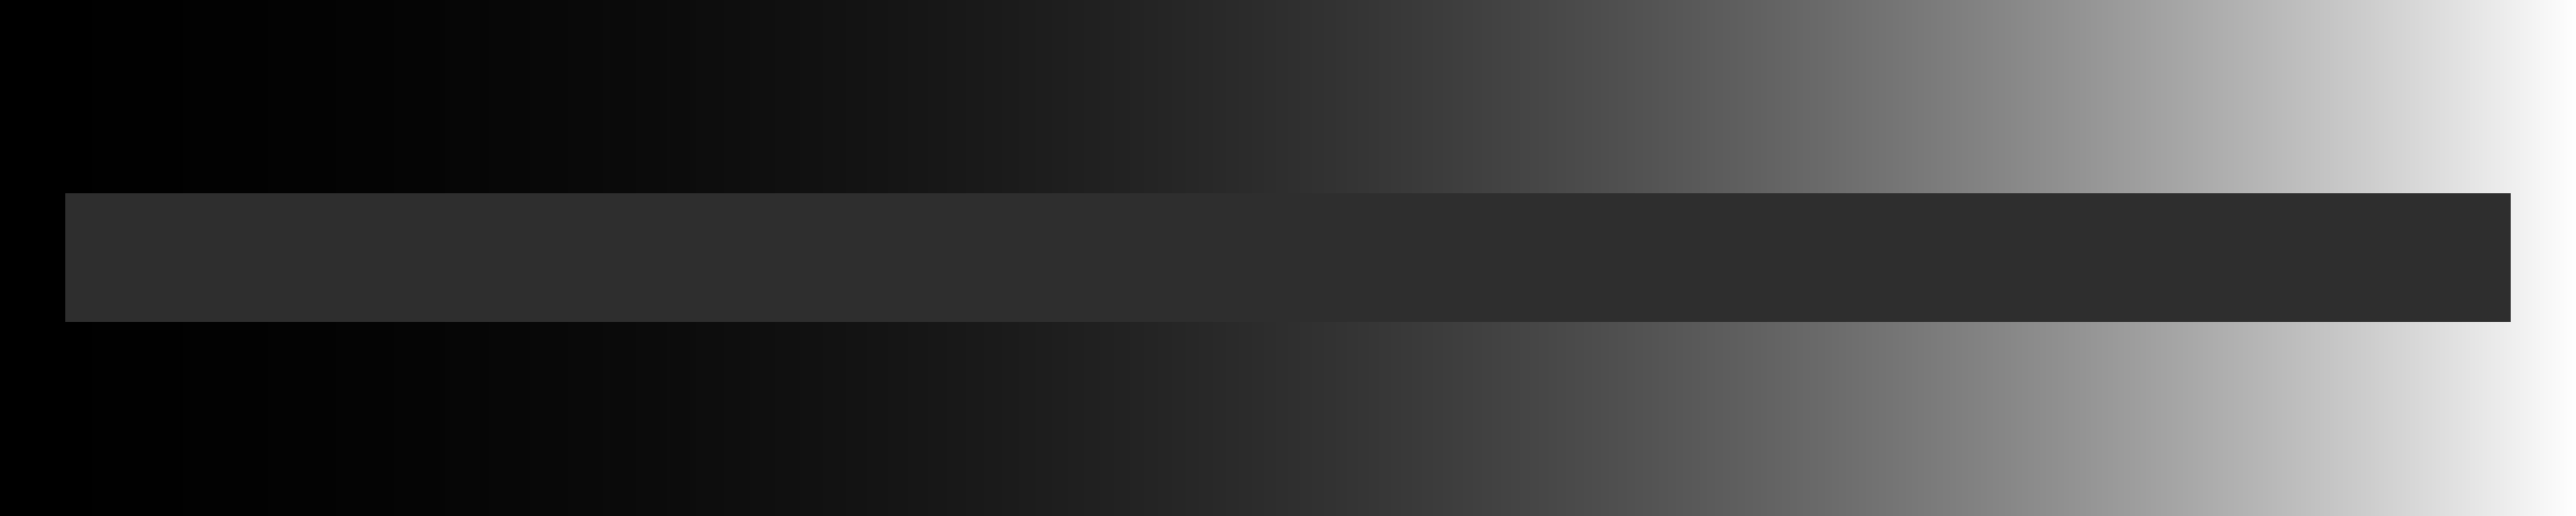
\includegraphics[width=2.5in]{images/GrayscaleLocality} \\
    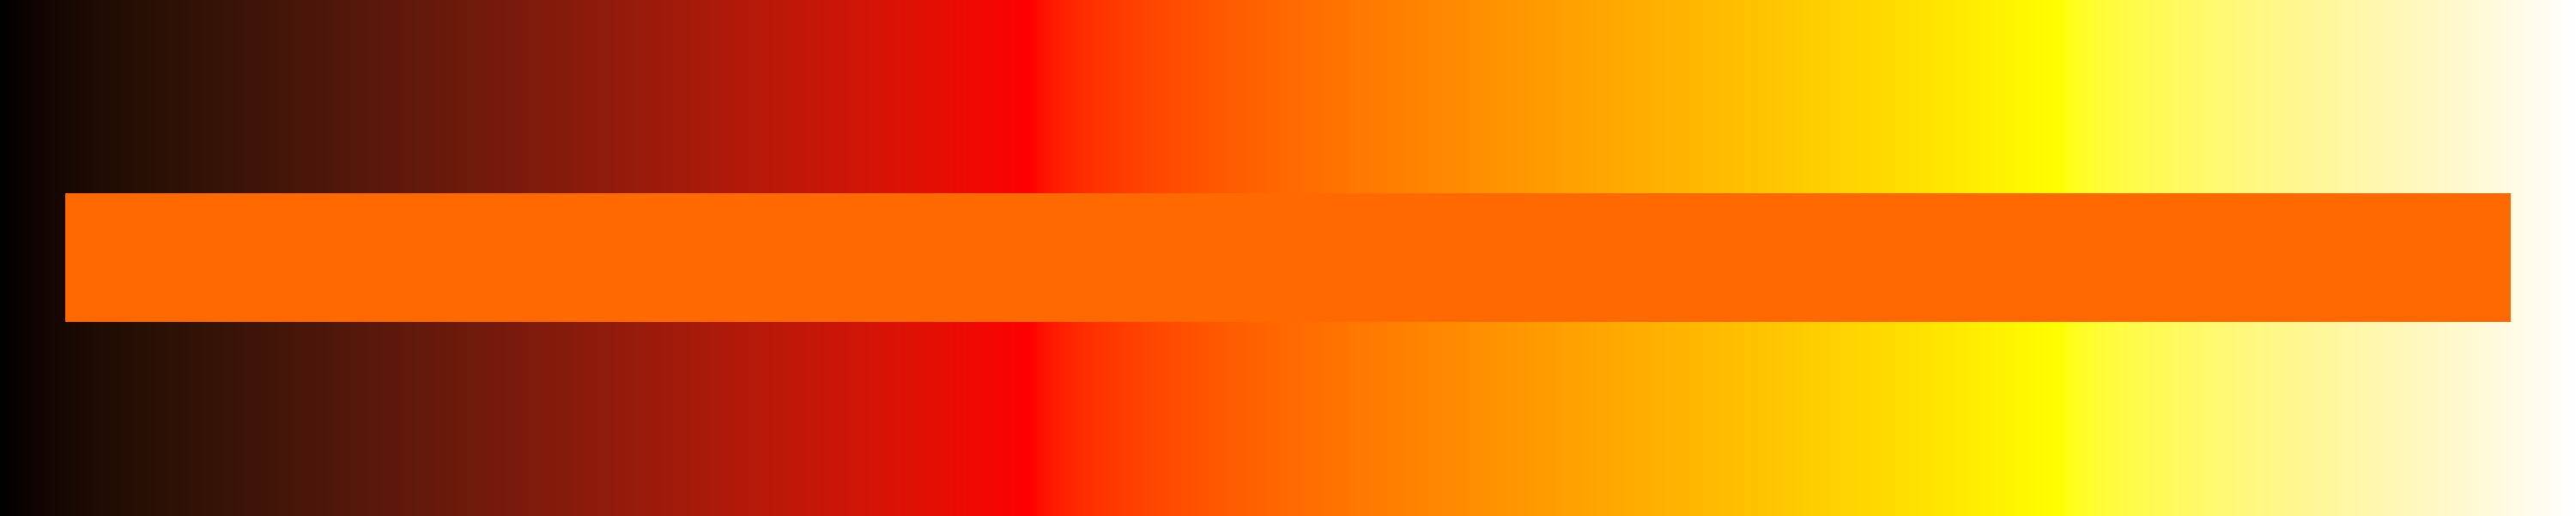
\includegraphics[width=2.5in]{images/BlackBodyLocality}
  \end{tabular}
  \caption{Pixels of the same luminance may look different depending on the
    surrounding pixels.}
  \label{fig:SimultaneousContrast}
\end{figure}
The grayscale color map also has disadvantages.  One problem is
that a human's perception of brightness is subject to the brightness of the
surrounding area.  Thus, when asked to compare the luminance of two objects
separated by distance and background, human subjects err up to 20\%.
This effect, demonstrated in Figure~\ref{fig:SimultaneousContrast}, is
called simultaneous contrast\lcite{Stone05}.  Adding a chromaticity shift
helps, but does not fix the problem entirely.  A chromatic shift also has
the possitive side effect of increasing the dynamic range of the color
map.

%% Simultaneous contrast still occurs, but the shift in chromaticity can help
%% resolve that.  Simultaneous color contrast can also occur, but can be
%% managed by changes in color opponent channels.

Another problem with grayscale color maps that is of greater concern for
general purpose scientific visualization is its interference with surface
shading.  The shading of 3D surfaces based on light sources is of utmost
importance for perceiving surface shape.  These shading cues are
composed almost entirely of luminance shifts.  Thus the luminance shift of
the grayscale color map masks the surface luminance shifts, especially in
the darker part of the spectrum, as demonstrated in
Figure~\ref{fig:LuminanceVsShading}.  The problem cannot be corrected
without a major reduction in the range that the luminance shifts in the color
map.

\begin{figure}
  \centering
  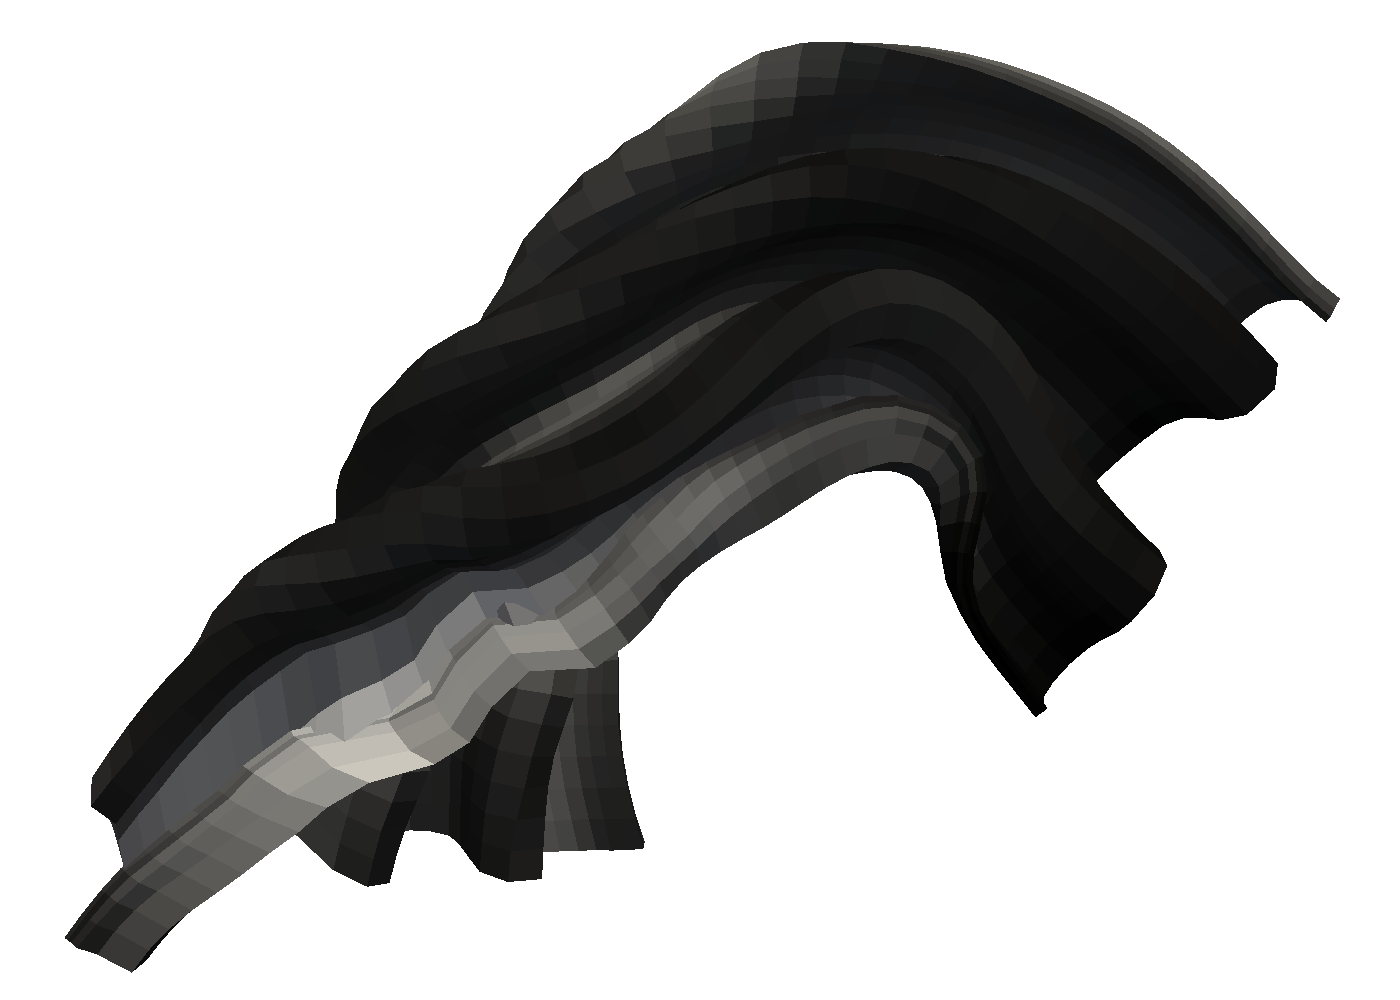
\includegraphics[width=1.25in]{images/GrayscaleShading}
  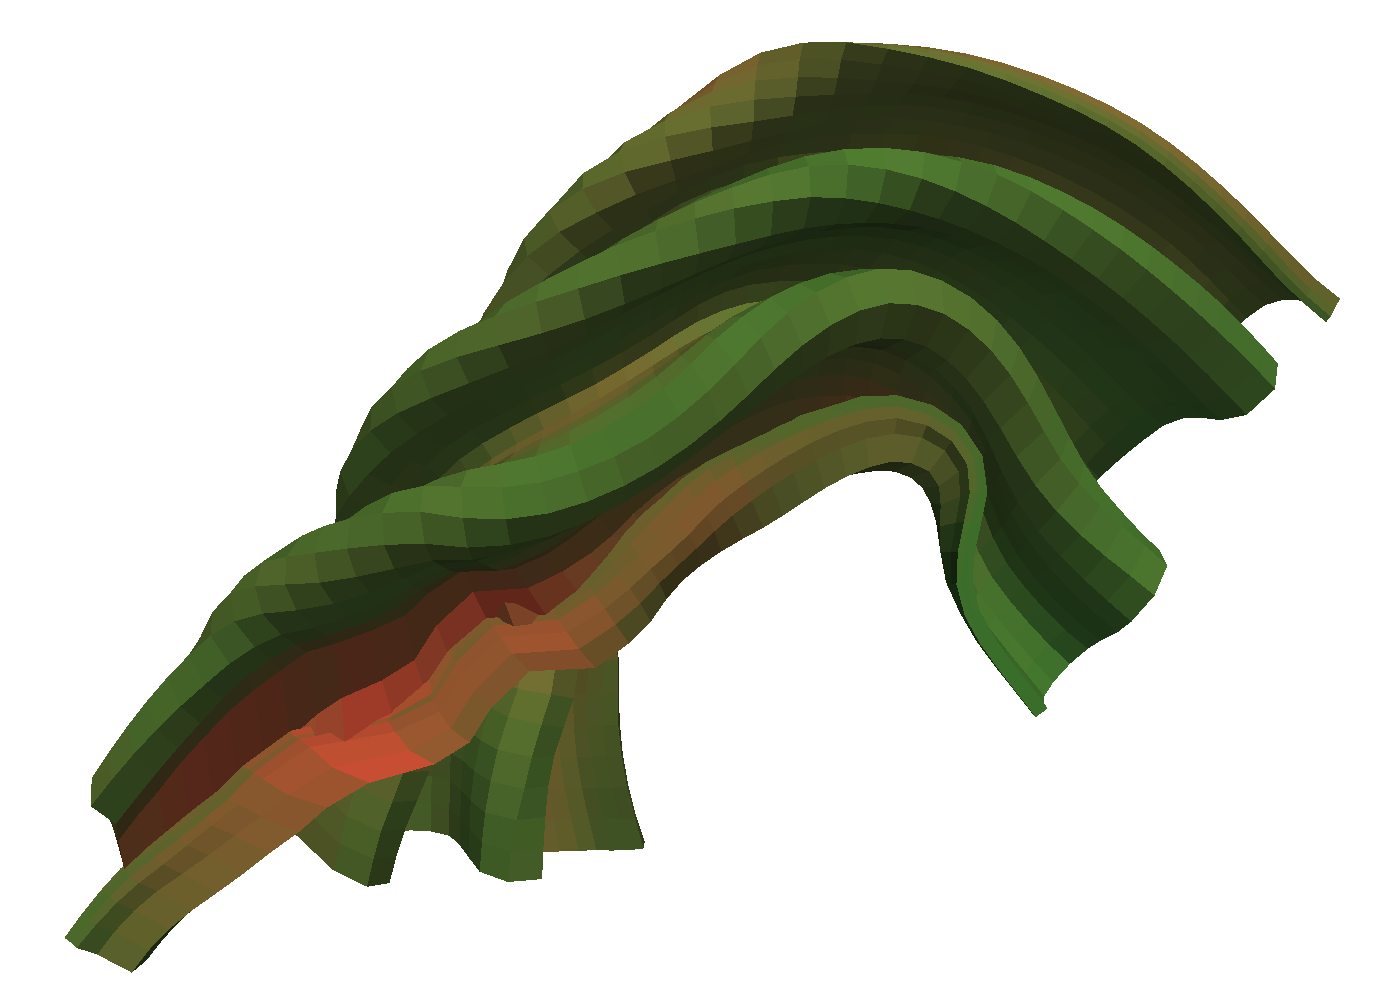
\includegraphics[width=1.25in]{images/Green2RedShading}
  \caption{Maps with big changes in luminance hide shading cues important
    for determining 3D structure (left image), whereas isoluminant maps
    minimize shading interference (right image).}
  \label{fig:LuminanceVsShading}
\end{figure}

\begin{figure}
  \centering
  \begin{tabular}{c}
    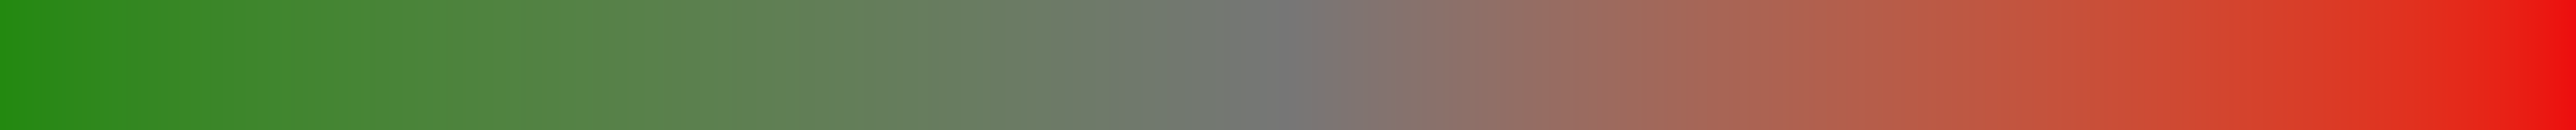
\includegraphics[width=2.5in]{images/Green2RedBar} \\
    
\includegraphics[width=2.5in]{images/Cyan2MauveBar}
  \end{tabular}
  \caption{Isoluminant color maps.  The green to red color map is popular
    because it uses a pair of opponent colors, but the cyan to mauve color
    map is much easier to see by individuals with deuteranope or protanopic
    vision.}
  \label{fig:IsoluminantColorMap}
\end{figure}
Another type of color map that is often suggested for use with 3D surfaces
is an isoluminant color map such as those demonstrated in
Figure~\ref{fig:IsoluminantColorMap}.  Somewhat opposite to the grayscale
map, an isoluminant map maintains a constant (perceptual) luminance and
relies entirely on chromatic shifts.  An isoluminant color map is
theoretically ideal for mapping onto shaded surfaces, as is demonstrated in
Figure~\ref{fig:LuminanceVsShading}.

Isoluminant color maps are not without their flaws, however.  Human
perception is less sensitive to changes in saturation or hue than changes
in luminance, especially for high frequency data\lcite{Rogowitz96}.
Holding the luminance constant also restricts the colors that can be
represented.  Thus, the isoluminant color map will have a lower fidelity
than one in which the luminance is allowed to change.  Isoluminant color
maps also tend to look dull and ugly, so casual users rarely
choose one over a more vibrant color map such as the rainbow color map.

These color maps comprise those most commonly used in the literature and tools
today.  Other color maps are proposed by Ware\scite{Ware04} as well as
several others.  Most are similar in spirit to those here with uniform
changes in luminance, saturation, hue, or some combination thereof.

\subsection{Color Spaces}
\label{sec:PreviousWork:ColorSpaces}

All color spaces are based on the tristimulus theory, which states that any
perceived color can be uniquely represented by a
3-tuple\lcite{Stone03}.  This result is a side effect
of the fact that there are exactly 3 different types of color receptors in
the human eye.  Limited space prevents more than a few applicable additive
color spaces from being listed here.  Any textbook on color will provide
more spaces in more detail\lcite{Stone03,Wyszecki82}.

The color space most frequently used in computer applications is the \RGB
color space.  This color space is adopted by many graphics packages such as
OpenGL and is presented to users by nearly every computer application
that provides a color chooser.  The three values in the \RGB
color space refer to the intensity output of each of the three light colors
used in a monitor, television, or projector.

Although it is often convenient to use \RGB to specify colors in terms of
the output medium, the display may have nonlinearities that interfere with
the blending and interpolation of colors\lcite{Stone03}.  When computing
physical light effects, it is best to use a color space defined by the
physical properties of light.  \XYZ is a widely used color space defined by
physical light spectra.  This conversion can be particularly difficult due
to differences between displays that make the color definition somewhat
ambiguous\lcite{Fortner97}.  For the purposes of this paper, we will assume
the \RGB space conforms to the canonical monitor defined by the sRGB
specification, a standard of the International Electrotechnical Commission
(IEC 61966-2-1) that is widely used by many color management
programs\lcite{Stone03}.  The conversion from the sRGB components to \RGB
components with physically linear properties is given in Equation~\ref{eqn:sRGB2linearRGB}.

\begin{equation}
  \begin{split}
    R_\mathrm{Linear} &=
    \begin{cases}
      \left((R_\mathrm{sRGB}+0.055)/1.055\right)^{2.4}
      & \text{if $R_\mathrm{Linear} > 0.04045$} \\
      R_{\mathrm{sRGB}}/12.92 & \text{otherwise}
    \end{cases} \\
    G_\mathrm{Linear} &=
    \begin{cases}
      \left((G_\mathrm{sRGB}+0.055)/1.055\right)^{2.4}
      & \text{if $G_\mathrm{Linear} > 0.04045$} \\
      G_{\mathrm{sRGB}}/12.92 & \text{otherwise}
    \end{cases} \\
    B_\mathrm{Linear} &=
    \begin{cases}
      \left((B_\mathrm{sRGB}+0.055)/1.055\right)^{2.4}
      & \text{if $B_\mathrm{Linear} > 0.04045$} \\
      B_{\mathrm{sRGB}}/12.92 & \text{otherwise}
    \end{cases} 
  \end{split}
  \label{eqn:sRGB2linearRGB}
\end{equation}

Given \RGB values that are linear with respect to physical light intensity,
conversion to \XYZ space is a simple linear transformation.  The
transformation is dependent on the characteristics of the display for which
the \RGB space is defined, but the sRGB specification yeilds the one in
Equation~\ref{eqn:rgb2xyz}.

\begin{equation}
  [X \quad Y \quad Z] = [R \quad G \quad B]
  \begin{bmatrix}
    0.4124 & 0.2126 & 0.0193 \\
    0.3576 & 0.7152 & 0.1192 \\
    0.1805 & 0.0722 & 0.9505
  \end{bmatrix}
  \label{eqn:rgb2xyz}
\end{equation}

There is a nonlinear relationship between light intensity and color
perception.  When defining a color map, we are more
interested in how a color is perceived than how it is formed.  In these
cases, it is better to use a color map based on how humans perceive color.
\Lab and \Luv are two common spaces.  The choice between the two is fairly
arbitrary; this paper uses \Lab.  The conversion from \XYZ to \Lab is given
in Equation~\ref{eqn:xyz2lab}.

\begin{equation}
  \begin{gathered}
    \begin{aligned}
      L* &= 116 \left[ \operatorname{f}(Y/Y_n) - 16/116 \right] \\
      a* &=
        500 \left[ \operatorname{f}(X/X_n) - \operatorname{f}(Y/Y_n) \right] \\
      b* &=
        200 \left[ \operatorname{f}(X/X_n) - \operatorname{f}(Y/Y_n) \right] \\
    \end{aligned} \\
    \operatorname{f}(x) \equiv
    \begin{cases}
      x^{1/3}          & \text{if $x > 0.008856$} \\
      7.787 x + 16/116 & \text{if $x \leq 0.008856$}
    \end{cases} \\
    [X_n \quad Y_n \quad Z_n] \text{ is a reference white value}
  \end{gathered}
  \label{eqn:xyz2lab}
\end{equation}

\Lab is an approximation of how humans perceive light.  The Euclidean
distance between two points is the approximate perceived difference between
the two colors.  This Euclidean distance in \Lab space is known as \DeltaE
and makes a reasonable metric for comparing color differences\lcite{Wyszecki82}.
This paper uses the notation $\DeltaE\{\cvec{c_1},\cvec{c_2}\}$ to denote
the \DeltaE for the pair of colors $\cvec{c_1}$ and $\cvec{c_2}$.


\section{Color Map Requirements}
\label{sec:ColorMapRequirements}

Our ultimate goal is to design a color map that works well for
general-purpose scientific visualization and a wide
variety of tasks and users.  As such we have the following requirements.
These criteria conform to many of those proposed
previously\lcite{Fortner97,Levkowitz92,Light04}.

\begin{itemize}
\item The map yields images that are aesthetically pleasing.
\item The map has a maximal perceptual resolution.
\item Interference with the shading of 3D surfaces is minimal.
\item The map is not sensitive to vision deficiencies.
\item The order of the colors should be natural and intuitively the same
  for all people.
\item The perceptual interpolation matches the underlying scalars the map
  represents.
\end{itemize}

The reasoning behind most of these requirements is self explanatory.  The
requirement that the color map be ``pretty,'' however, is not one often
found in the scientific literature.  After all, the attractiveness of the
color map, which is difficult to quantify in the first place, has little to
do with its effectiveness in conveying information.  Nevertheless, aesthetic
appeal is important as users will use that as a criterion in selecting
visualization products and generating images.

% \begin{itemize}
% \item Due to the proliferation of visualization programs and images using
%   the rainbow color map, many users will have ``learned'' the order of the
%   colors and will continue to have to use them.  Our color map should try
%   not to break that convention.
% \item Color maps often co-exist with other visible elements: labels,
%   backgrounds, auxiliary structures and features, annotation, etc.  Thus,
%   the color map should yield well other elements with carefully chosen
%   colors.
% \end{itemize}

Several of these requirements are contradictory, making the choice of a
general purpose color map difficult.  All of the examples in
Section~\ref{sec:PreviousWork:ColorMaps} excel in some of the requirements,
but fail completely in one or more of the others.  It is impossible to have
a color map that performs perfectly against all of the requirements.  Our color
map must be a compromise that works reasonably well in all areas.


\section{Color Map Design}
\label{sec:ColorMapDesign}

There are many color maps in existence today, but very few of them satisfy
all of the requirements listed in Section~\ref{sec:ColorMapRequirements}.
For inspiration, I turn to the field of cartography.  People
have been making maps for thousands of years, and throughout this history
there has been much focus on both the effectiveness of
conveying information as well as the aesthetics of the design.

Brewer\scite{Brewer05} provides excellent advice for designing cartographic
color maps and many well-designed examples.\footnote{Brewer's color maps
are also available on her web site:
\href{http://www.colorbrewer.org}{www.colorbrewer.org}.} Brewer divides her
color maps into three classes: qualitative, sequential, and diverging.
Examples of these color maps are shown in Figure~\ref{fig:BrewerExamples}.

\begin{figure}
  \centering
  \subfigure[Qualitative]{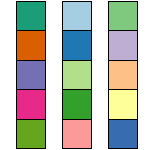
\includegraphics{images/ColorMapsQualitative}}
  \quad
  \subfigure[Sequential]{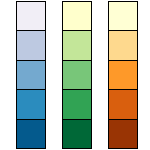
\includegraphics{images/ColorMapsSequential}}
  \quad
  \subfigure[Diverging]{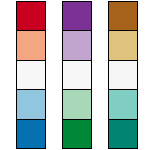
\includegraphics{images/ColorMapsDiverging}}
  \caption{Examples of color maps from Brewer\scite{Brewer05}.}
  \label{fig:BrewerExamples}
\end{figure}

The qualitative color maps (also known as nominal color maps\lcite{Ware04})
are used to represent a collection of discrete, unordered classes.  Since
the colors have no ordering (by design), they are not appropriate for
mapping a scalar variable.

The sequential color maps (also known as ordinal\lcite{Ware04} or
saturation\lcite{Rheingans99} color maps) are (nearly) monochromatic.  They
range from a heavily saturated color to various levels of unsaturation.
Luminance is also often increased as saturation is decreased so that the
color map terminates in a color at or close to white.  The monotonic nature
of the saturation level maps well to a scalar value.
% Sequential maps are
% usually oriented such that the most saturated color represents the lowest
% scalar value whereas the more luminant white represents the highest scalar
% value.  However, the color map, which has a limited range of luminance, can
% sometimes be flipped.  For example, if a red or orange sequential color map
% represented temperature, it would be more natural to represent the highest
% temperature with the most saturated color.

The diverging color maps (also known as ratio\lcite{Ware04},
bipolar\lcite{Spence01}, or double-ended\lcite{Rheingans99}) have two major
color components.  The map transitions from one color component to the
other by passing through an unsaturated color (white or yellow).  Diverging
color maps are typically used to represent a scalar with a significant
value at or near the median.  For example, a color map for elevation could
put sea level at white with below sea level in blue and above sea level in
tan\lcite{Tufte97}.  The ordering of the colors is usually based on the
context within which they are used.

Sequential color maps are clearly appropriate for scientific visualization.
Their monotonic nature maps well to scalar values.  Diverging color maps
are a less obvious choice.  We cannot expect there to be some significant
median value that the diverging color map is designed to highlight.

However, diverging color maps can better satisfy the requirements given in
Section~\ref{sec:ColorMapRequirements} than their sequential counterparts.
First, the more colorful nature of the diverging color map can be more
aesthetically pleasing.  Second, the diverging color map can have up to
twice the perceptual resolution of the sequential color map without
sacrificing the requirements of surface shading or losing viewers
with dichromatic vision.  Furthermore, the diverging color map visually
divides scalar values into three logical regions: low, midrange, and high
values.  These regions provide more visual cues that are helpful for
understanding data.

What diverging color maps lack in general is a natural ordering of colors.
To impose a color ordering, we carefully chose two colors that most
naturally have ``low'' and ``high'' connotations.  We achieve this with the
concept of ``cool'' and ``warm'' colors.

Studies show that people identify red and yellow colors as warm and blue and
blue-green colors as cool across subjects, contexts, and
cultures.  Furthermore, people associate warmth with positive activation
and coolness with negative activation\lcite{Hardin97}.  Consequently,
mapping cool blues to low values and warm reds to high values is
natural\lcite{Fortner97}.


\subsection{Perceptual Uniformity}
\label{sec:PerceptualUniformity}

An important characteristic of any color map is that it is perceptually
uniform throughout.  For a discrete color map, perceptual uniformity means
that all pairs of adjacent colors will look equally different from each
other.  That is, the \DeltaE for each adjacent pair is (roughly) the same.

For a continuous color map, we want the perceptual distance between two
colors to be proportional to the distance between the scalars associated
with each.    If we characterize our color map with function $\cvec{c}(x)$
that takes scalar value $x$ and returns a color vector, the color map is
perceptually uniform if
\begin{equation}
  \frac{\DeltaE\{\cvec{c}(x),\cvec{c}(x+\Delta{x})}{\Delta{}x}
  \label{eq:StrictContinuousDE}
\end{equation}
is constant for all valid $x$.

Strictly speaking, we cannot satisfy Equation~\ref{eq:StrictContinuousDE}
for diverging color maps because the map necessarily passes through three
points in \Lab space that are not in a line.  However, it is possible to
ensure that the rate of change is constant.  That is,
\begin{equation}
  \lim_{\Delta{}x \rightarrow 0}{
    \frac{\DeltaE\{\cvec{c}(x),\cvec{c}(x+\Delta{x})}{\Delta{}x} }
  \label{eq:ContinuousDE}
\end{equation}
is constant for all valid $x$.  This relaxed property is sufficient for
describing a perceptually linear color map so long as we make sure that the
curve does not return to any set of colors.

We can resolve Equation~\ref{eq:ContinuousDE} a bit by applying the \DeltaE
operation and splitting up the $\cvec{c}$ function into its components.
\begin{equation}
  \begin{split}
    { \lim_{\Delta x \rightarrow 0}
      \frac{\left\lVert \cvec{c}(x+\Delta x) - \cvec{c}(x) \right\rVert}
      {\Delta x}} \\
    { \lim_{\Delta x \rightarrow 0}
      \left\lVert \frac{\cvec{c}(x+\Delta x)- \cvec{c}(x)}
	  {\Delta x} \right\rVert } \\
    { \lim_{\Delta x \rightarrow 0}
      \sqrtsign{ \sum_i \left( \frac
	  {\operatorname{c}_i(x+\Delta x)
	    - \operatorname{c}_i(x)}
	  {\Delta x} \right)^2 } } \\
    {\sqrtsign{ \sum_i \left( \lim_{\Delta x \rightarrow 0}
       \frac
	  {\operatorname{c}_i(x+\Delta x)
	    - \operatorname{c}_i(x)}
	  {\Delta x} \right)^2 } }
  \end{split}
  \label{eqn:dE_limit}
\end{equation}

In the final form of Equation~\ref{eqn:dE_limit}, we can clearly see that
the limit is the definition of a derivative.  So replacing the limit with a
derivative, we get the following.

\begin{equation}
  \sqrtsign{\sum_i (\operatorname{c}_{i}'(x))^2}
  \label{eqn:dE_comp_dif}
\end{equation}

With some abuse of notation, let us declare $\cvec{c}'(x)$ as the piecewise
derivative of $\cvec{c}(x)$.  Using this notation,
Equation~\ref{eqn:dE_comp_dif} clearly resolves to the following.

\begin{equation}
  \left\lVert \cvec{c}'(x) \right\rVert
  \label{eqn:dE}
\end{equation}

The easiest way to ensure that Equation~\ref{eqn:dE} is constant
is to linearly interpolate colors in the \Lab color space.  However, that
is not entirely possible to do for diverging color maps.  Lines from red to
blue will not go through white.  A piecewise linear interpolation is mostly
effective, but can create an artificial Mach band at white where the
luminance sharply transitions from increasing to decreasing as demonstrated
in Figure~\ref{fig:LinearMachBands}.

\begin{figure}
  \centering
  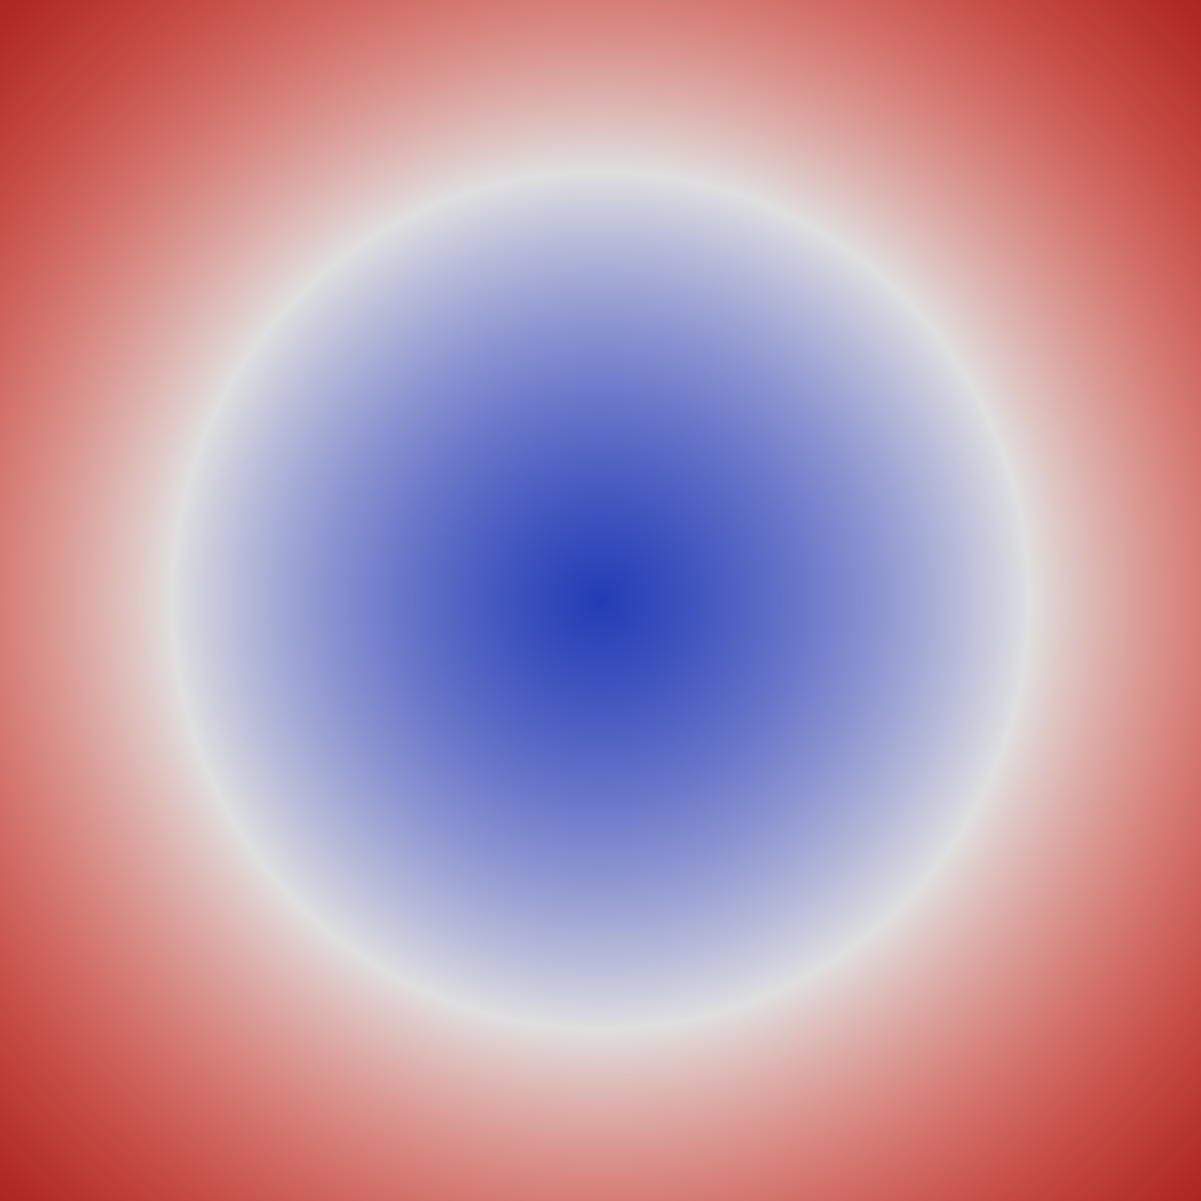
\includegraphics[width=1in]{images/Cool2WarmLabRadial}
  \qquad
  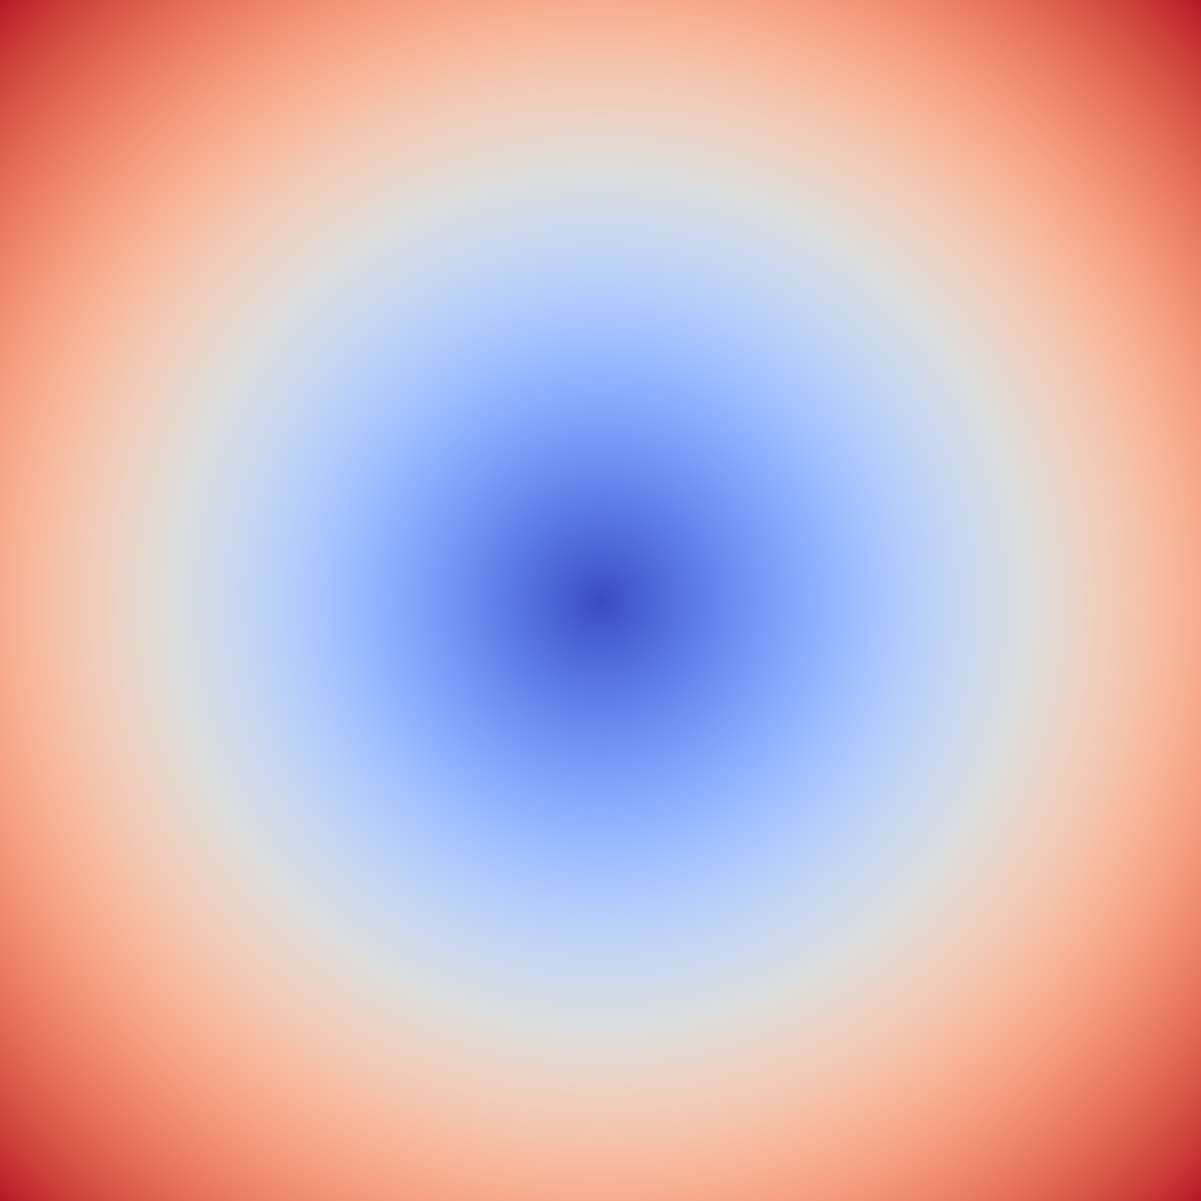
\includegraphics[width=1in]{images/Cool2WarmRadial}
  \caption{Using piecewise linear interpolations in \Lab color space causes
    Mach bands in the white part of diverging color maps (left image).  The
    transition can be softened by interpolating in \Msh space (right image).}
  \label{fig:LinearMachBands}
\end{figure}

Rather than have a sharp transition in the luminance, we require a
``leveling off'' of the luminance as the color map approaches white.  To
compensate, the chromaticity must change more dramatically in this part of
the color map.  A method for designing this type of color map is defined in
the next section.

\subsection{\Msh Color Space}
\label{sec:MshColorSpace}

To simplify the design of continuous, diverging color maps, I derive a new
color space called \Msh.  \Msh is basically a polar form of the \Lab color
space.  $M$ is the magnitude of the vector, $s$ (the saturation) is the
angle away from the $L*$ axis, and $h$ (the hue) is the angle of the
vector's projection in the $a*$-$b*$ plane.  Conversion between the two
color spaces is straightforward.

\begin{equation}
  \begin{split}
    M &= \sqrt{{L*}^2 + a*^2 + b*^2} \\
    s &= \arccos \frac{L*}{M} \\
    h &= \arctan \frac{b*}{a*}
  \end{split}
  \label{eqn:LabToMsh}
\end{equation}

\begin{equation}
  \begin{split}
    L* &= M \cos s \\
    a* &= M \sin s \cos h \\
    b* &= M \sin s \sin h
  \end{split}
  \label{eqn:MshToLab}
\end{equation}

Note that \Msh, like all polar coordinates, has a pole in which one of the
coordinates is ill defined.  Specifically, when $s = 0$ (the color is on
the $L*$ axis), $h$ has no effect.  This pole was chosen because it
coincides with a singularity in human vision.  When saturation is low, the
color has no hue.  It is therefore possible to make a discontinuous jump
in the hue while still maintaining perceptual continuance.

Piecewise linear interpolations in \Msh space behave very well for
diverging color maps.  As $s$ linearly approaches zero, the luminance
naturally levels out while the chromaticity changes faster.
% Although this
% will lead to a more significant rate of change in the chromaticity, it will
% not be noticeable as it coincides with a singularity in perception.  In
% fact, we can make a jump in the value of the hue at that point without it
% being noticeable.

An ideal way to build a diverging color map in \Msh space is to start at
one color, linearly reduce $s$ to 0 (to get white), flip $h$ to the
appropriate value for the last color, and then linearly increase $s$ to the
desired value.  In fact, we can show that if $s$ changes linearly while $M$
and $h$ are held constant, Equation~\ref{eqn:dE} is constant, which is our
criterion for a uniform color map.  We can characterize a $\cvec{c}(x)$ that
behaves in this way in \Lab space as
\begin{equation}
  \cvec{c}(x) = [ M \cos \operatorname{s}(x) \quad
  M \sin \operatorname{s}(x) \cos h \quad
  M \sin \operatorname{s}(x) \sin h ]
  \label{eqn:s_linear}
\end{equation}
where $M$ and $h$ are constant and $\operatorname{s}(x)$ is a linear
function of slope $s_m$.

Now we can plug Equation~\ref{eqn:s_linear} into Equation~\ref{eqn:dE} and
resolve.

\begin{equation}
  \begin{gathered}
    \left\lVert M s_m \sin\operatorname{s}(x) \quad
        M s_m \cos\operatorname{s}(x) \cos h \quad
        M s_m \cos\operatorname{s}(x) \sin(h) \right\rVert \\
    \sqrtsign{ M^2 s_m^2 \left( \sin^2 \operatorname{s}(x)
        + \cos^2 \operatorname{s}(x) \cos^2 h
        + \cos^2 \operatorname{s}(x) \sin^2 h \right) } \\
    \sqrtsign{ M^2 s_m^2 \left( \sin^2 \operatorname{s}(x)
        + \cos^2 \operatorname{s}(x) \left( \cos^2 h
          + \sin^2 h \right) \right) } \\
    \sqrtsign{ M^2 s_m^2 \left( \sin^2 \operatorname{s}(x)
        + \cos^2 \operatorname{s}(x) \right) } \\
    M s_m
    \label{eqn:s_linear_uniform}
  \end{gathered}
\end{equation}

Clearly Equation~\ref{eqn:s_linear_uniform} resolves to a constant and
therefore meets our criterion for a ``uniform'' color space.  There is still
a discontinuity when we flip $h$.  However, because this discontinuous
change of hue occurs when there is no saturation, it is not noticeable.
And unlike the piecewise linear interpolation in \Lab space, this piecewise
linear interpolation in \Msh space results in a smooth change in luminance
throughout the entire color map, as evidenced in Figure~\ref{fig:s_plot}.

\begin{figure}
  \centering
  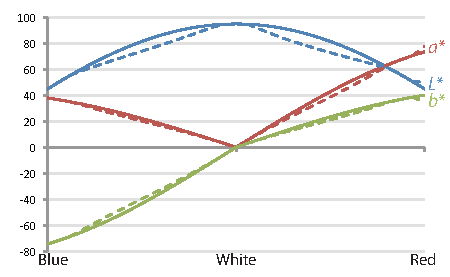
\includegraphics{images/LinearMshPlot}
  \caption{Plot of $L*$, $a*$, and $b*$ coordinates when interpolating $s$
    linearly in \Msh space.  Dashed lines show effect when colors are
    ``clipped'' to the gamut of a typical monitor. \sticky{Fix color conversion.}}
  \label{fig:s_plot}
\end{figure}

Although the color map shape shown in Figure~\ref{fig:s_plot} has good
visual properties, it does not conform well to the gamut of colors
displayable by a video monitor.  When trying to display many of these
colors, you must ``clip'' to what can be represented (demonstrated by the
dashed lines).  Notice the harsh bends of the intensity ($L*$) that occur
near the middle.  These bends can lead to Mach banding.  We can correct for
this problem by reducing $M$ at each end, but this adds the problem that
colors will change faster near white when $M$ is larger.

We can restore the uniformity of the color map again by adding some
``spin'' to the hue.  Even though $h$ is interpolated linearly, the changes
have a greater effect on the color when $s$ is larger, which can
counterbalance the growing $M$.  The next section describes how to chose an
appropriate hue change.

\subsection{Choosing a Hue Spin}
\label{sec:ChoosingAHueSpin}

Let us consider the transition from a saturated color, $\cvec{c}_s=(M_s,
s_s, h_s)$, at an end of the color map to an unsaturated ``white'' color,
$\cvec{c}_u=(M_u, 0, h_u)$, at the middle of the color map.  As the
color map moves from $\cvec{c}_s$ to $\cvec{c}_u$, the $M$, $s$, and $h$
coordinates are varied linearly.  The slope of these coordinates can be
characterized as $M_m = M_u - M_s$, $s_m = -s_s$, and $h_m = h_u - h_s$.
(Note that $h_u$ has no effect on the unsaturated color, but is provided to
conveniently define the rate of change.)

\begin{figure}
  \centering
  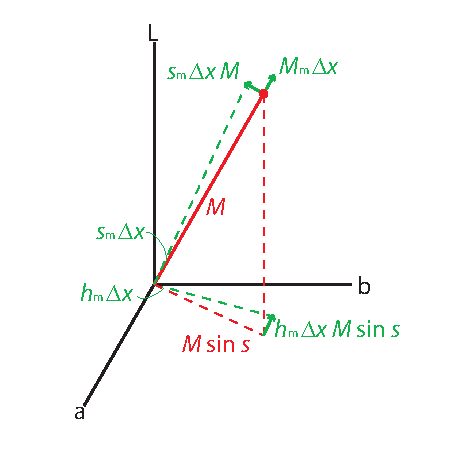
\includegraphics[height=2in]{images/MshDeltaMovements}
  \caption{A small linear movement in \Msh space}
  \label{sec:LinearMshMovement}
\end{figure}

Figure~\ref{sec:LinearMshMovement} shows how a small movement in this
linear \Msh function behaves in \Lab space.  The distance measurements take
advantage of the property that if you rotate a vector of radius $r$ by some
small angle $\Delta\alpha$, then the change in the vector is
$\lim_{\Delta\alpha \rightarrow 0}r \Delta\alpha$.  Clearly the \DeltaE,
the magnitude of change in \Lab space, is
\begin{equation}
  \sqrt{(M_m \Delta x)^2 + (s_m \Delta x M)^2 + (h_m \Delta x M \sin s)^2}
  \label{eq:DeltaEforLinearMshMovement}
\end{equation}

Equation~\ref{eq:DeltaEforLinearMshMovement} will not be constant unless
$M_m$ and $h_m$ are zero, which, as described in the previous section, is
unacceptable.  However we can get pretty close to constant by choosing
$h_u$ so that Equation~\ref{eq:DeltaEforLinearMshMovement} is equal for
$\cvec{c}_s$ and $\cvec{c}_u$.

\begin{multline}
  \sqrt{(M_m \Delta x)^2 + (s_m \Delta x M_s)^2 + (h_m \Delta x M_s \sin s_s)^2}
  \\ =
  \sqrt{(M_m \Delta x)^2 + (s_m \Delta x M_u)^2}
  \label{eqn:hm_criterion}
\end{multline}

Note that the right side of Equation~\ref{eqn:hm_criterion} is missing a
term because it evaluates to 0 for the unsaturated color.  We can safely
get rid of the square roots because there is a sum of square real numbers
inside them both.

\begin{align}
    (M_m \Delta x)^2 + (s_m M_s)^2 \quad & \notag \\
    + (h_m M_s \sin s_s)^2 &= (M_m \Delta x)^2 + (s_m M_u)^2 \notag \\
    h_m^2 M_s^2 \sin^2 s_s &= s_m^2 (M_u^2 - M_s^2) \notag \\
    h_m^2 &= \frac{s_m^2 (M_u^2 - M_s^2)}{M_s^2 \sin^2 s_s} \notag \\
    h_m &= \pm \frac{s_m \sqrt{M_u^2 - M_s^2}}{M_s \sin s_s}
    \label{eqn:adjusted_hm}
\end{align}

Remember that $s_m=-s_s$.  We can use Equation~\ref{eqn:adjusted_hm} to
determine a good hue to use for the white point (from the given side).

\begin{equation}
  h_u = h_s \pm \frac{s_s \sqrt{M_u^2 - M_s^2}}{M_s \sin s_s}
  \label{eqn:adjusted_hu}
\end{equation}

Note that Equation~\ref{eqn:adjusted_hu} will most certainly yield a
different value for each of the saturated colors used in the diverging
color map.  The direction in which the hue is ``spun'' is unimportant with
regard to perception.  I usually adjust the hue to be away from 0 (except
in the purple hues) because it provides slightly more aesthetically
pleasing results.  Figure~\ref{fig:AdjustHue} gives a simple algorithm for
adjusting the hue.

\begin{figure}
  \begin{codebox}
    \Procname{$\proc{AdjustHue}(\{M_\mathrm{sat},s_\mathrm{sat},
                                h_\mathrm{sat}\},M_\mathrm{unsat})$}
    \li \If $M_\mathrm{sat} \geq M_\mathrm{unsat}$
    \li \Then \Return $h_\mathrm{sat}$ \RComment Best we can do
    \li \Else $\id{hSpin} \leftarrow
                 \frac{s_\mathrm{sat}\sqrt{M_\mathrm{unsat}^2-M_\mathrm{sat}^2}}
		      {M_\mathrm{sat} \sin(s_\mathrm{sat})}$
    \li       \If $h_\mathrm{sat} > -\frac{\pi}{3}$ \RComment Spin away from purple
    \li       \Then \Return $h_\mathrm{sat} + \id{hSpin}$
    \li       \Else \Return $h_\mathrm{sat} - \id{hSpin}$
              \End
        \End
  \end{codebox}
  \caption{Function to provide an adjusted hue when interpolating to an
    unsaturated color in \Msh space.}
  \label{fig:AdjustHue}
\end{figure}

\begin{figure}
  \centering
  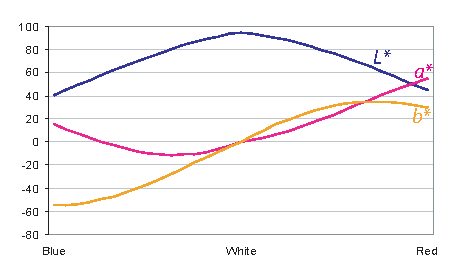
\includegraphics{images/HueSpinPlot}
  \caption{Plot of $L*$, $a*$, and $b*$ coordinates when interpolating
    piecewise linearly in \Msh space and applying a hue spin. \sticky{Fix
      to new colors.}}
  \label{fig:hue_spin_plot}
\end{figure}

Figure~\ref{fig:hue_spin_plot} shows the effects of applying a hue spin.
The plot is smooth, perceptually uniform, and comparable to the plot given
in Figure~\ref{fig:s_plot}.  In addition, the hue spin allows the entire
curve to remain in the gamut of displayable colors.


\subsection{Interpolating Control Points}
\label{sec:InterpolatingControlPoints}

\begin{figure}
  \begin{codebox}
    \Procname{$\proc{InterpolateColor}(\{r_1,g_1,b_1\},\{r_2,g_2,b_2\},
                                       \id{interp})$}
    \li $\{M_1,s_1,h_1\} \leftarrow \proc{RGB2Msh}(\{r_1,g_1,b_1\})$
    \li $\{M_2,s_2,h_2\} \leftarrow \proc{RGB2Msh}(\{r_2,g_2,b_2\})$
    \zi \Comment If points saturated and distinct, place white in middle
    \li \If $(s_1 > 0.05) \cap (s_2 > 0.05)
             \cap (\proc{RadDiff}(h_1,h_2) > \frac{\pi}{3})$
	\label{code:InterpolateColor:AddWhiteBegin}
    \li \Then $M_{\mathrm{mid}} \leftarrow \max(M_1,M_2,88)$
    \li       \If $\id{interp} < \frac{1}{2}$
    \li       \Then $M_2 \leftarrow M_{\mathrm{mid}}, s_2 \leftarrow 0, h_2 \leftarrow 0$
    \li             $\id{interp} \leftarrow 2\id{interp}$
    \li       \Else $M_1 \leftarrow M_{\mathrm{mid}}, s_1 \leftarrow 0, h_1 \leftarrow 0$
    \li             $\id{interp} \leftarrow 2\id{interp} - 1$
              \End
        \End
	\label{code:InterpolateColor:AddWhiteEnd}
    \zi \Comment Adjust hue of unsaturated colors
    \li \If $(s_1 < 0.05) \cap (s_2 > 0.05)$
        \label{code:InterpolateColor:AdjustHueBegin}
    \li \Then $h_1 \leftarrow \proc{AdjustHue}(\{M_2,s_2,h_2\},M_1)$
    \li \ElseIf $(s_2 < 0.05) \cap (s_1 > 0.05)$
    \li \Then $h_2 \leftarrow \proc{AdjustHue}(\{M_1,s_1,h_1\},M_2)$
        \End
	\label{code:InterpolateColor:AdjustHueEnd}
    \zi \Comment Linear interpolation on adjusted control points
    \li $\{M_\mathrm{mid},s_\mathrm{mid},h_\mathrm{mid}\}$
    \zi \>$\leftarrow (1-\id{interp})\{M_1,s_1,h_1\}+\id{interp}\{M_2,s_2,h_2\}$
        \label{code:InterpolateColor:LinearInterpolate}
    \li \Return $\proc{Msh2RGB}(\{M_\mathrm{mid},s_\mathrm{mid},h_\mathrm{mid}\})$
  \end{codebox}
  \caption{Interpolation algorithm to automatically create continuous
    diverging color maps.}
  \label{fig:InterpolateColor}
\end{figure}

The \proc{InterpolateColor} algorithm in Figure~\ref{fig:InterpolateColor}
combines the techniques described previously in this section.  The
algorithm simplifies the process of building a continuous diverging color
map by allowing a user to define colors at control points.
\proc{InterpolateColor} accepts two colors and an interpolation factor
between $0$ and $1$.  \proc{InterpolateColor} takes colors in \RGB space to
make it easier for users to define.

The \proc{InterpolateColor} algorithm works as follows.  The colors are
first converted to \Msh.\footnote{The implementations of \proc{RGB2Msh} and
\proc{Msh2RGB} can be derived from Equations \ref{eqn:rgb2xyz},
\ref{eqn:xyz2lab}, \ref{eqn:LabToMsh}, and \ref{eqn:MshToLab}.}  To enforce
a diverging color map, white is added between the two control points
(lines~\ref{code:InterpolateColor:AddWhiteBegin}--\ref{code:InterpolateColor:AddWhiteEnd}).
The middle white points is not added if either color is already unsaturated
(indicating that there is already a control point for the white part of the
diverging color map) or if the angular difference between the two hue
orientations (computed by \proc{RadDiff}) is small (which would mean that
both sides of the diverging color map would be roughly the same
color).\footnote{The parameters for specifying a low saturation (less than
$0.05$ radians) and similar hue angles (less than $\frac{\pi}{3}$ radians)
is somewhat arbitrary, but the values provided here work well in practice.}
If either control point is unsaturated, its hue is adjusted
(lines~\ref{code:InterpolateColor:AdjustHueBegin}--\ref{code:InterpolateColor:AdjustHueEnd})
using the \proc{AdjustHue} function in Figure~\ref{fig:AdjustHue}.
Finally, the two \Msh colors are linearly interpolated
(line~\ref{code:InterpolateColor:LinearInterpolate}).  The result is
converted back to \RGB and returned.

The \proc{InterpolateColor} algorithm makes it easy for users to build and
modify continuous diverging color maps using \RGB control points as
demonstrated in Figure~\ref{fig:ColorMapInteraction}.

\begin{figure}
  \centering
  \begin{tabular}{c}
    \subfigure[Simply pick two endpoint colors to create a diverging color
      map in between them.]%
	      {%
		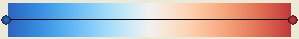
\includegraphics[width=.45\linewidth]{images/tfOriginal}\qquad%
		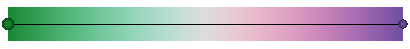
\includegraphics[width=.45\linewidth]{images/tfColorChange}
	      } \\
    \subfigure[Creating a white or gray control point allows you to define
      the intensity and location of the ``middle'' of the diverging color
      map.]%
	      {%
		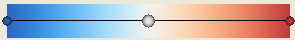
\includegraphics[width=.45\linewidth]{images/tfWhiteMiddle}%
		\qquad%
		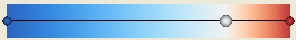
\includegraphics[width=.45\linewidth]{images/tfWhiteShifted}
	      } \\
    \subfigure[Adding a control point in a colored area allows you to
      stretch and compress regions.]%
	      {%
		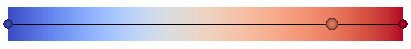
\includegraphics[width=.45\linewidth]{images/tfColorPoint}%
		\qquad%
		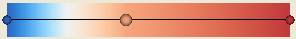
\includegraphics[width=.45\linewidth]{images/tfColorShifted}
	      }
  \end{tabular}
  \caption{Interacting with color maps in the \Msh color space.}
  \label{fig:ColorMapInteraction}
\end{figure}


\section{Results}
\label{sec:Results}

\begin{figure}
  \centering
  
\includegraphics[width=2.5in]{images/Cool2WarmBar}
  \caption{A continuous diverging color map that is well suited to scientific
    visualization.}
  \label{fig:Cool2WarmBar}
\end{figure}

\begin{figure*}
  \centering
  \begin{tabular}{c@{\;}c@{\;}c@{\;}c@{\;}c@{\;}c}
    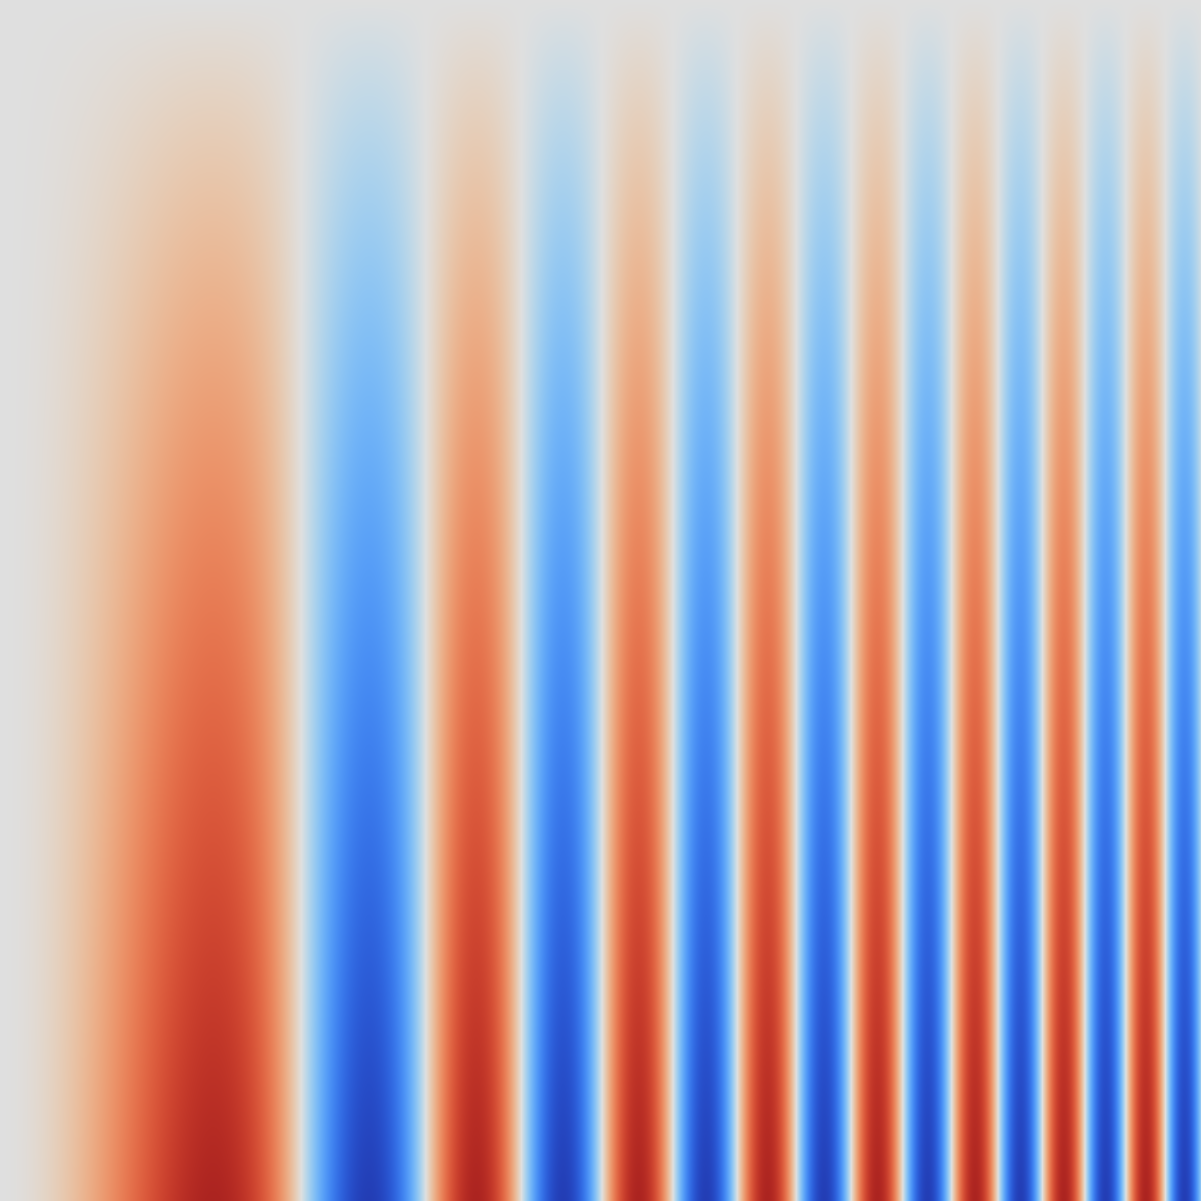
\includegraphics[width=1.1in]{images/Cool2WarmSpatialContrast} &
    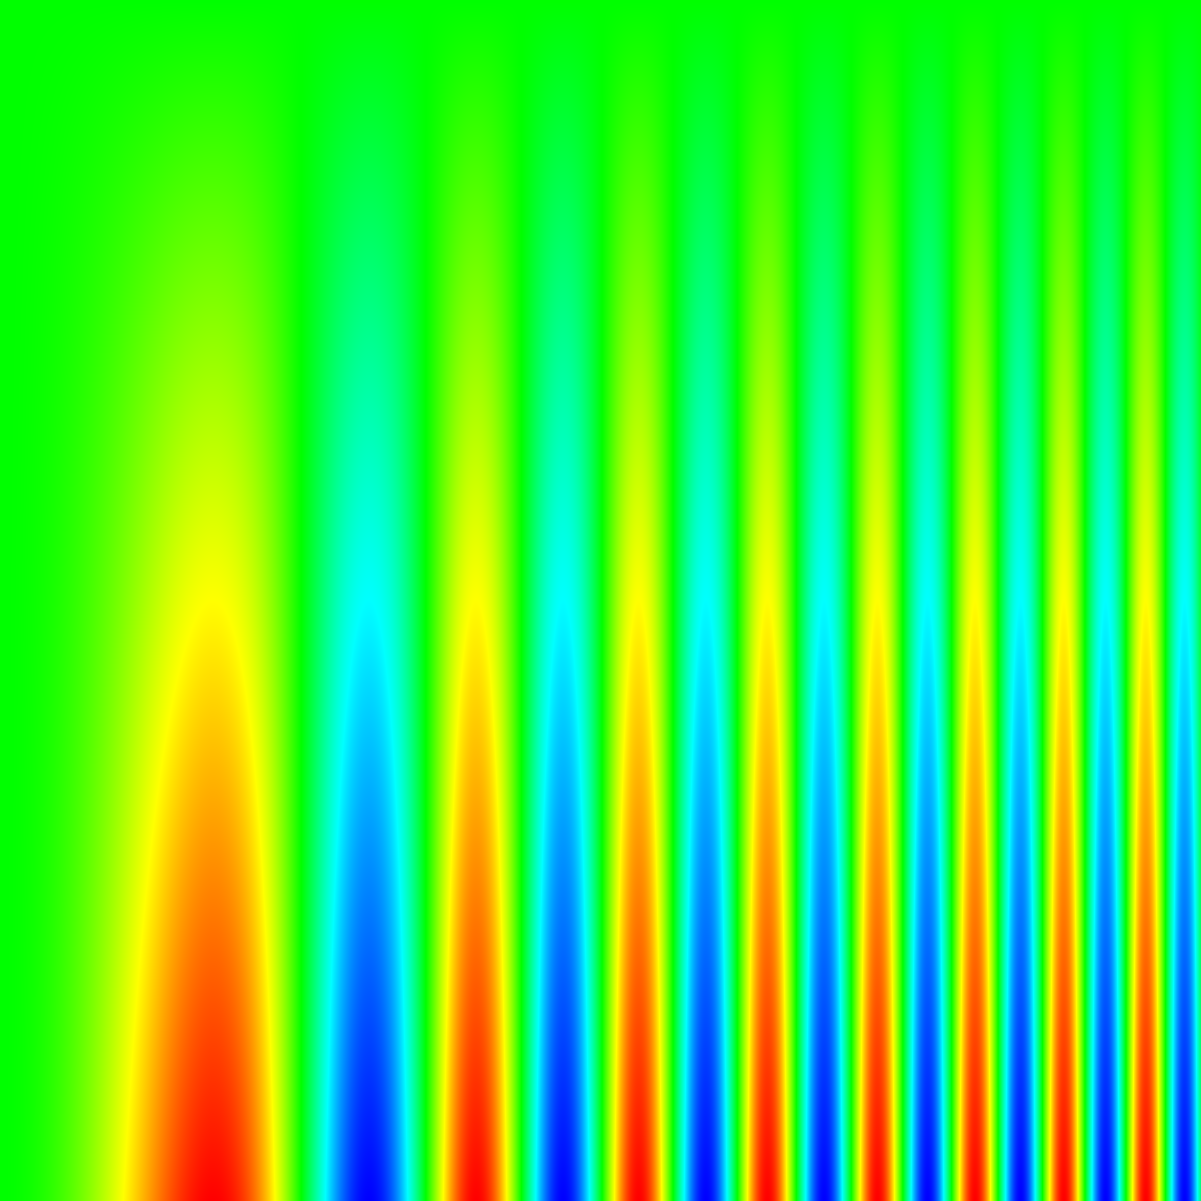
\includegraphics[width=1.1in]{images/RainbowSpatialContrast} &
    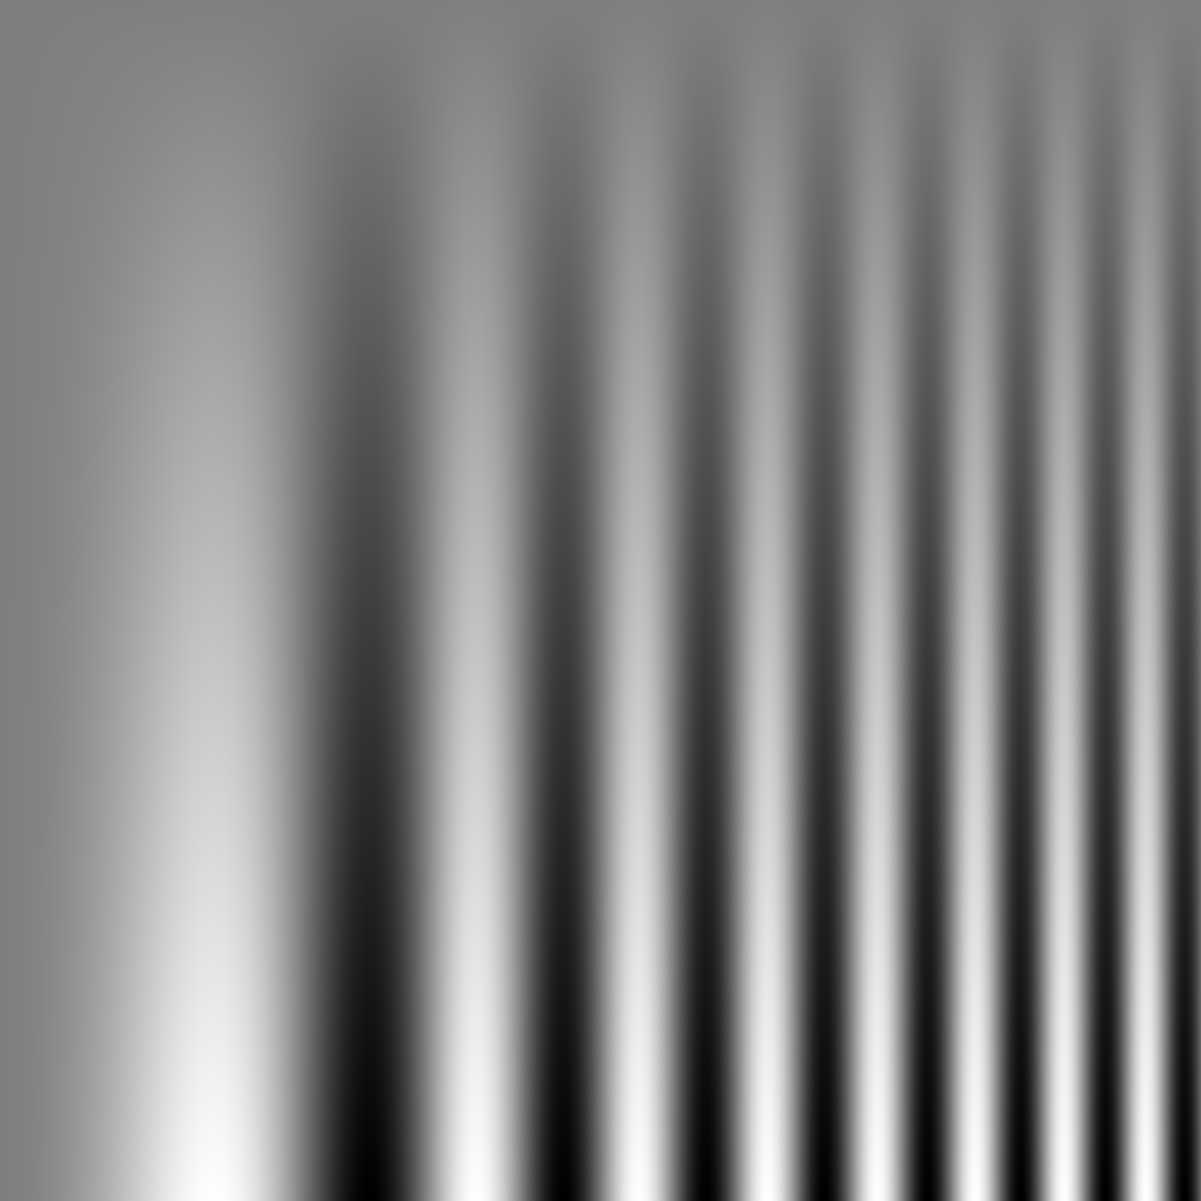
\includegraphics[width=1.1in]{images/GrayscaleSpatialContrast} &
    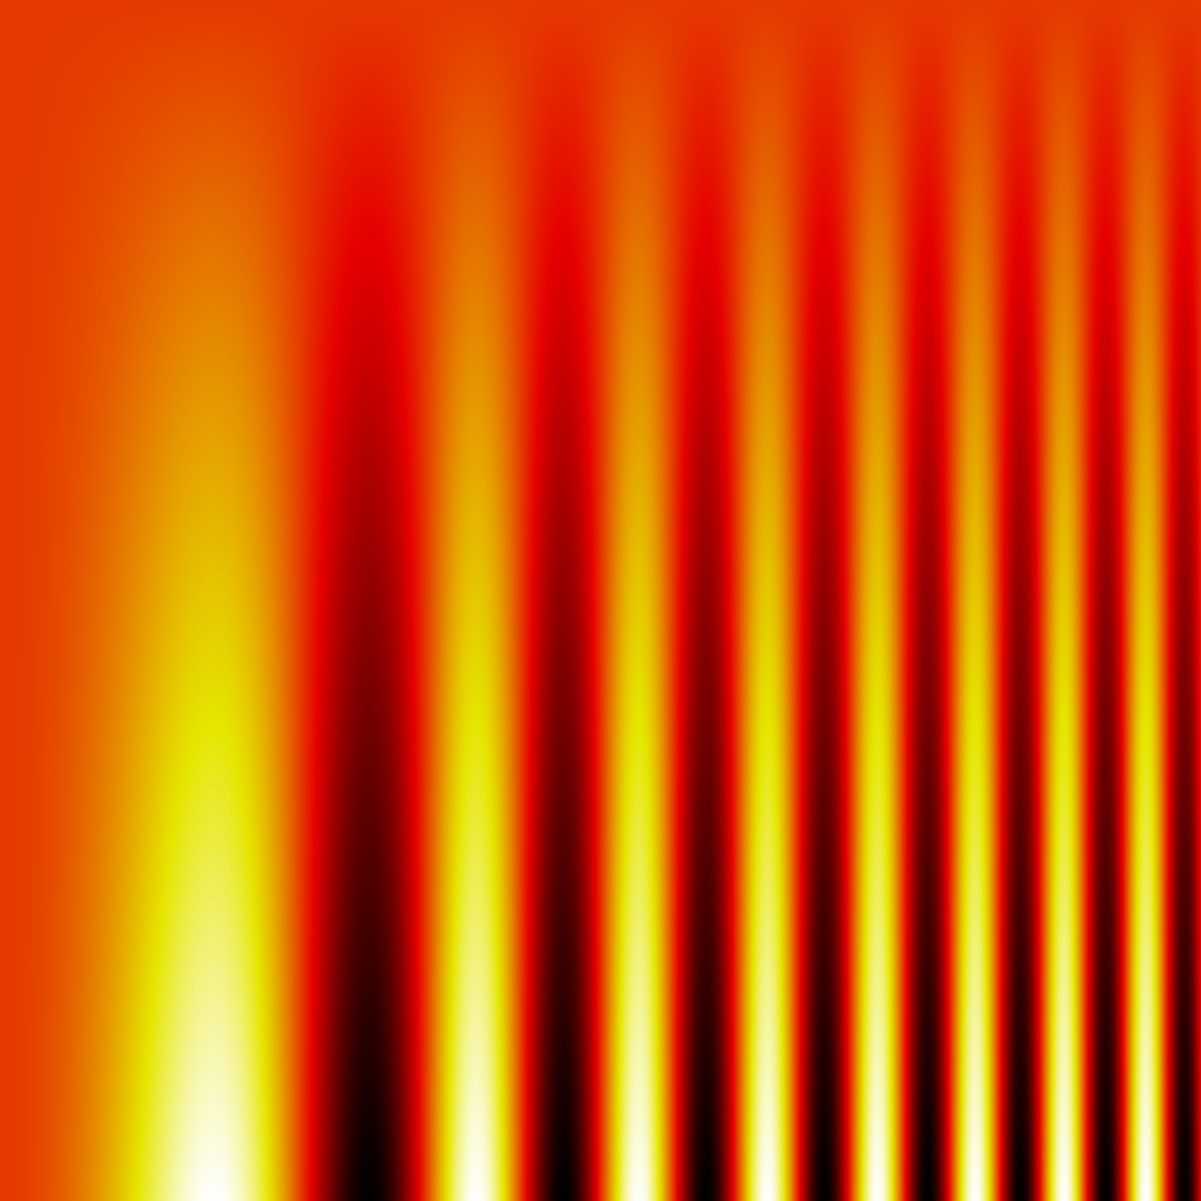
\includegraphics[width=1.1in]{images/BlackBodySpatialContrast} &
    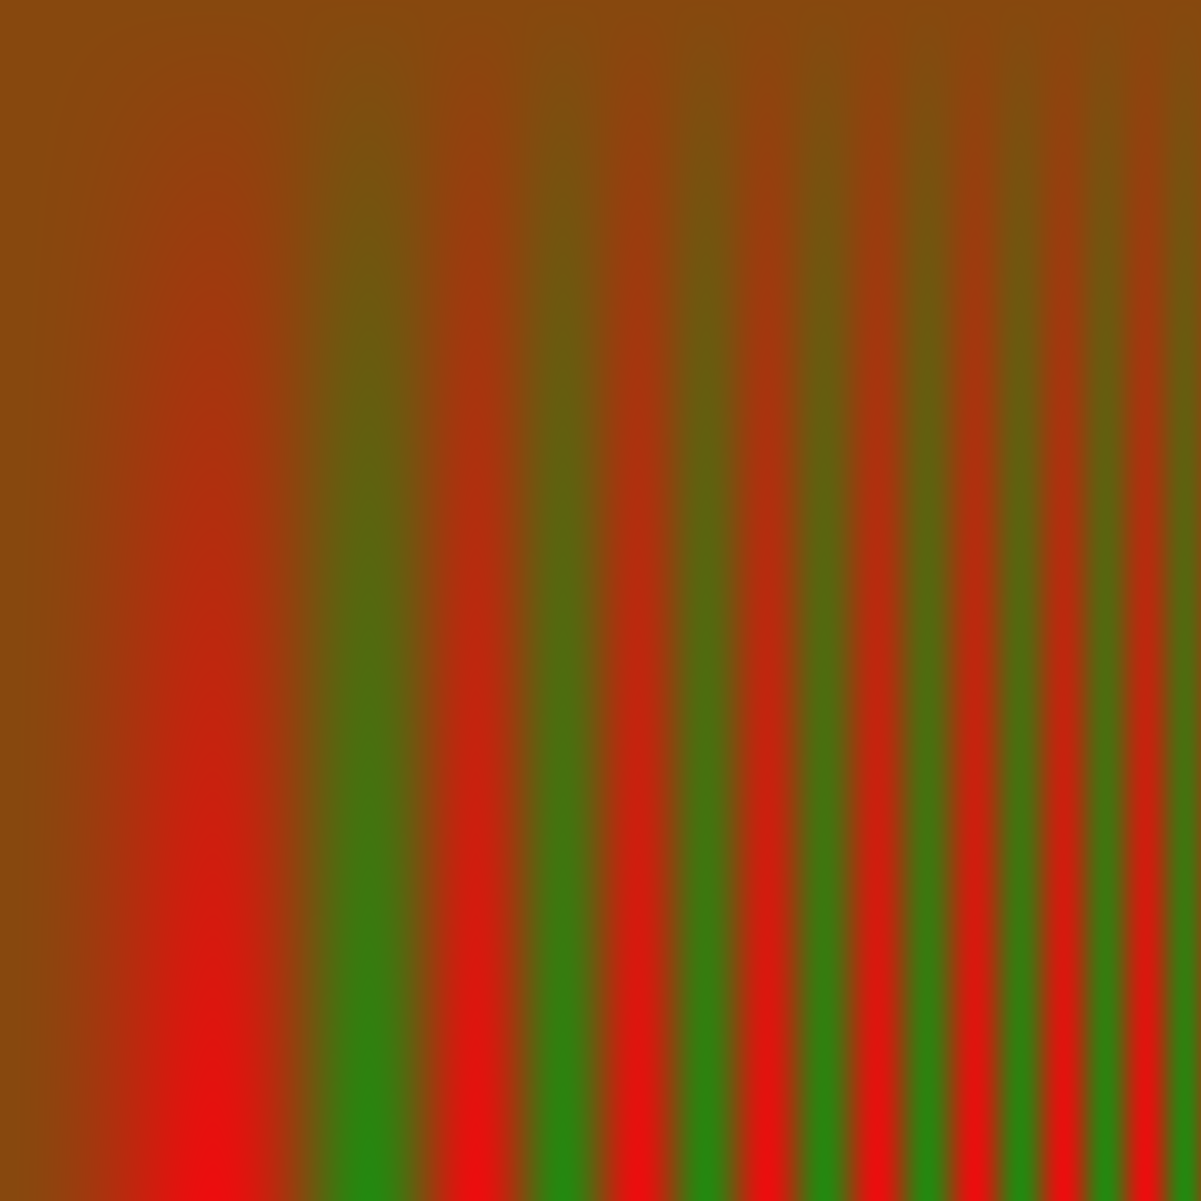
\includegraphics[width=1.1in]{images/Green2RedSpatialContrast} &
    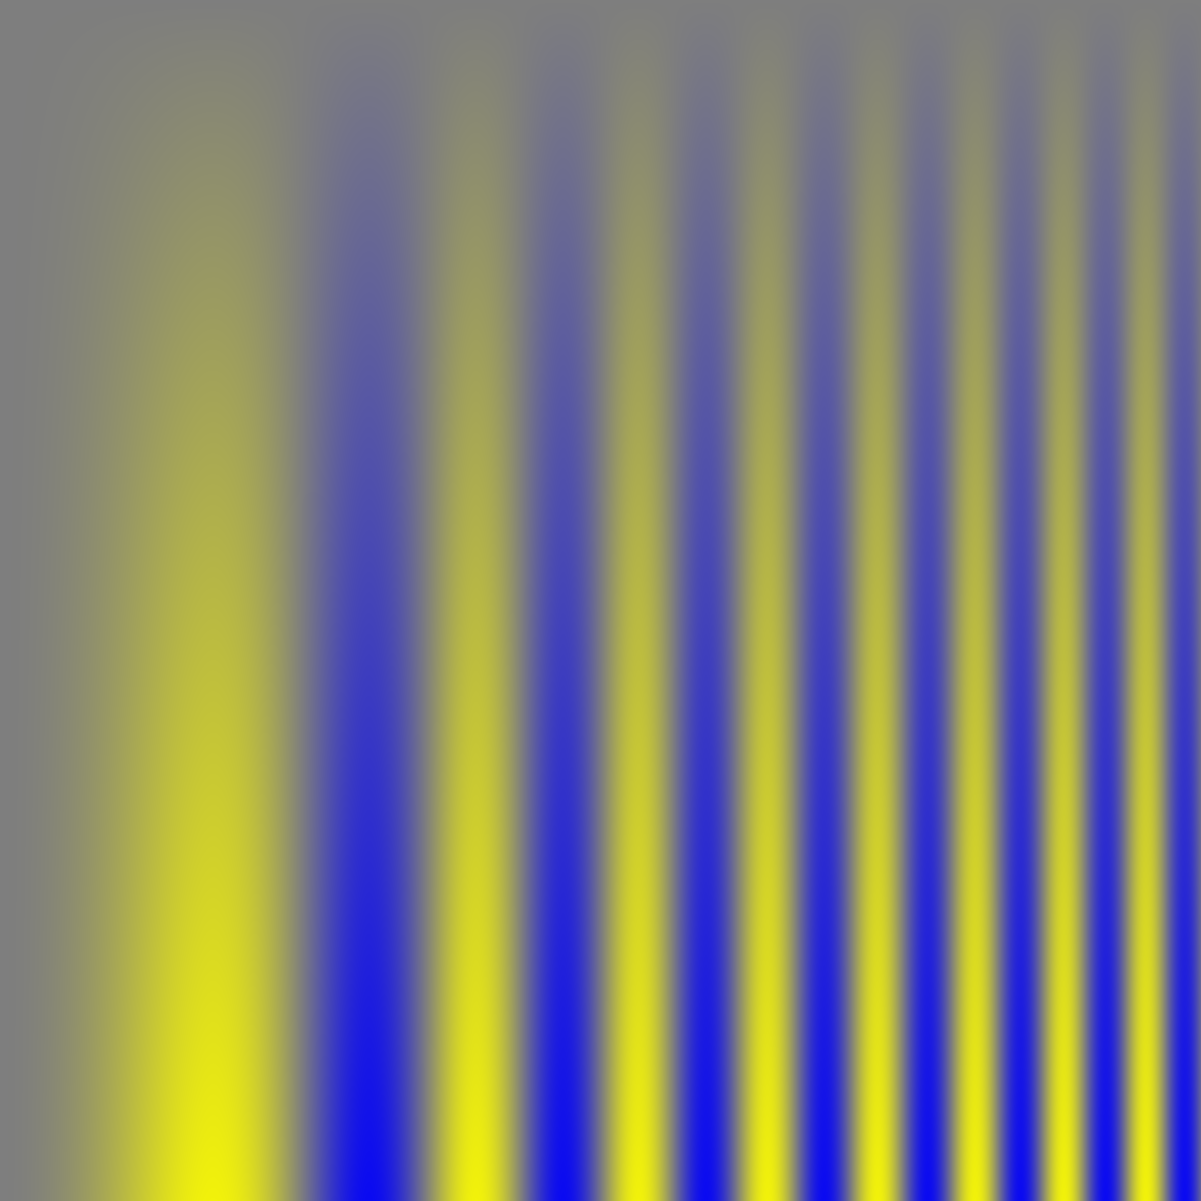
\includegraphics[width=1.1in]{images/Blue2YellowSpatialContrast} \\

    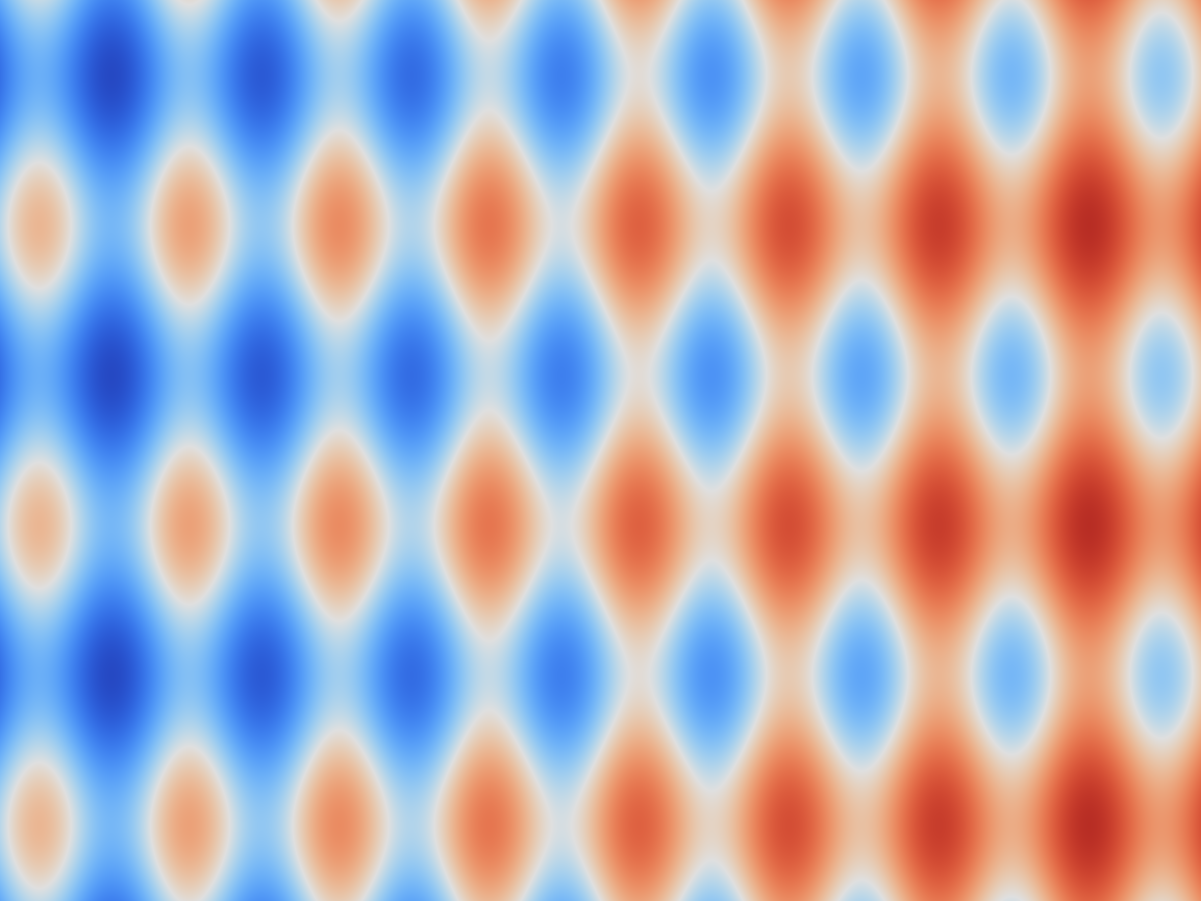
\includegraphics[width=1.1in]{images/Cool2WarmLfSensitivity} &
    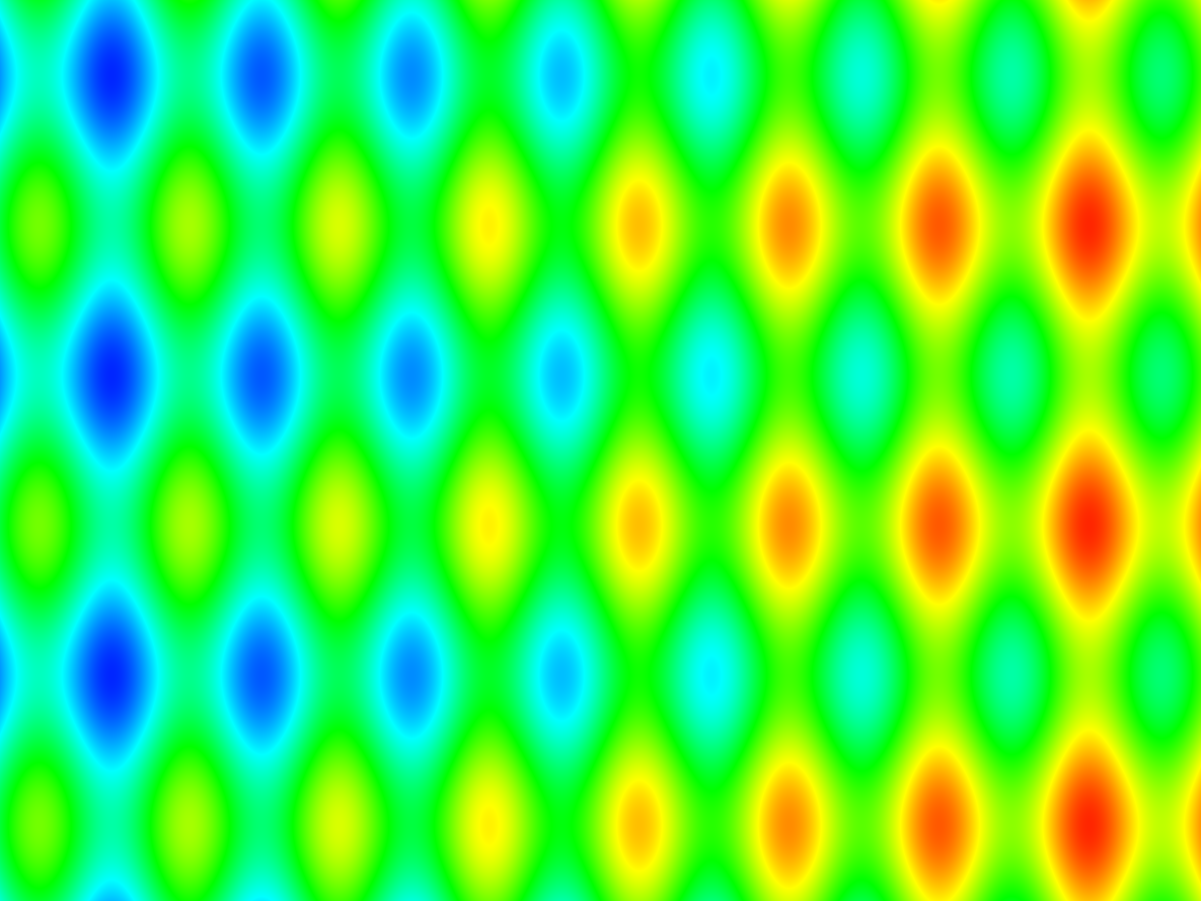
\includegraphics[width=1.1in]{images/RainbowLfSensitivity} &
    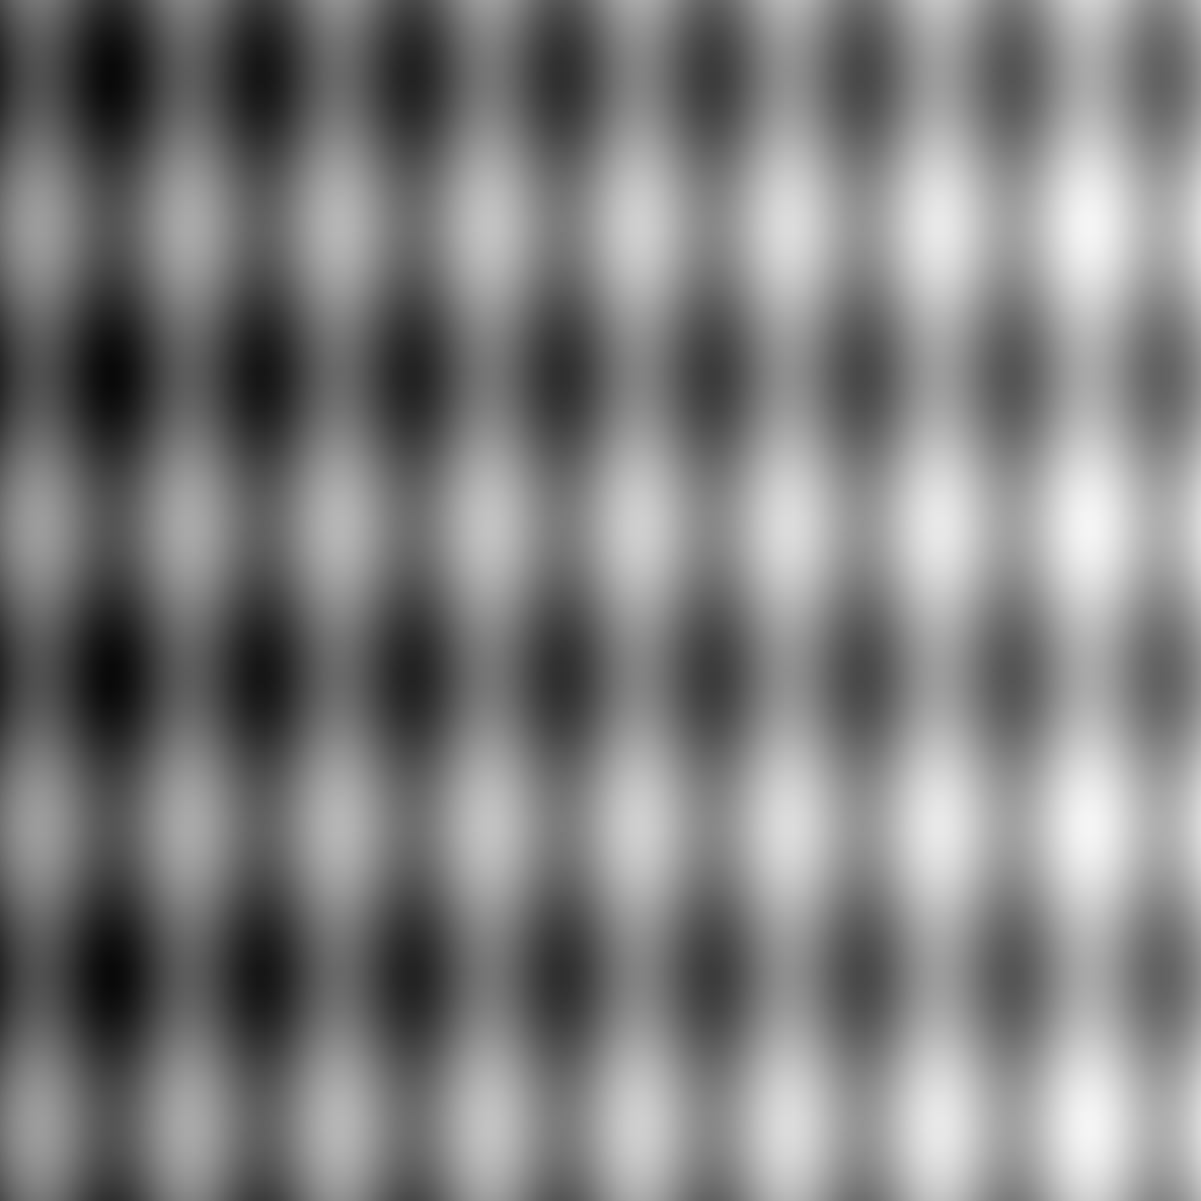
\includegraphics[width=1.1in]{images/GrayscaleLfSensitivity} &
    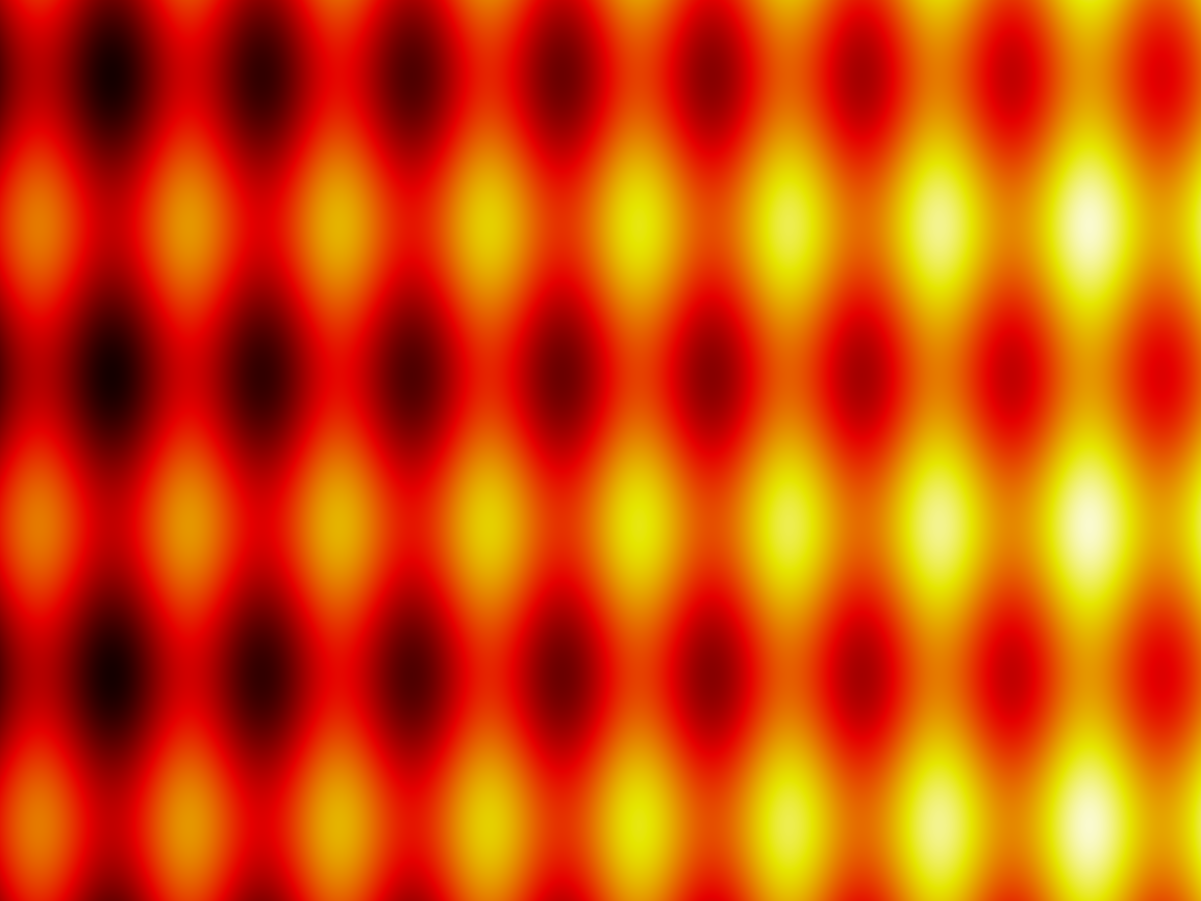
\includegraphics[width=1.1in]{images/BlackBodyLfSensitivity} &
    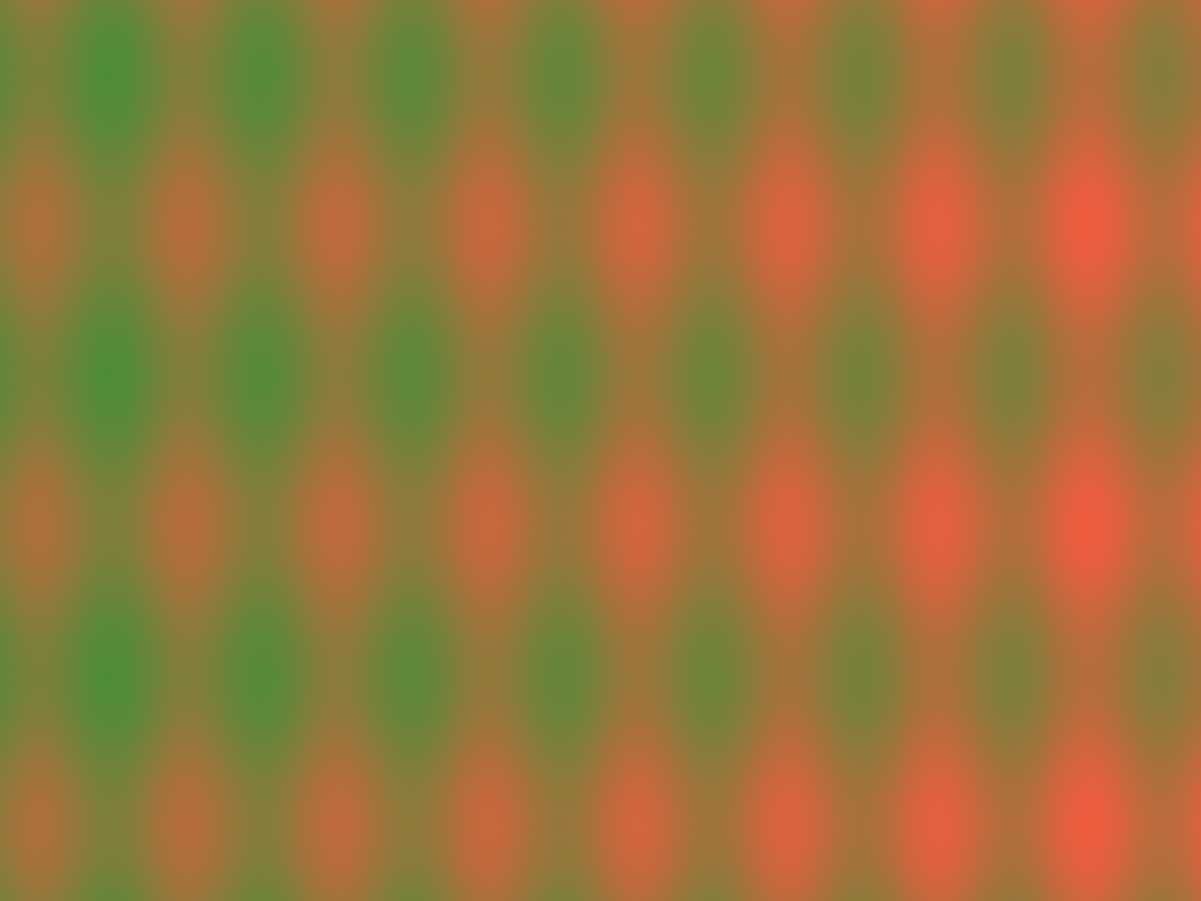
\includegraphics[width=1.1in]{images/Green2RedLfSensitivity} &
    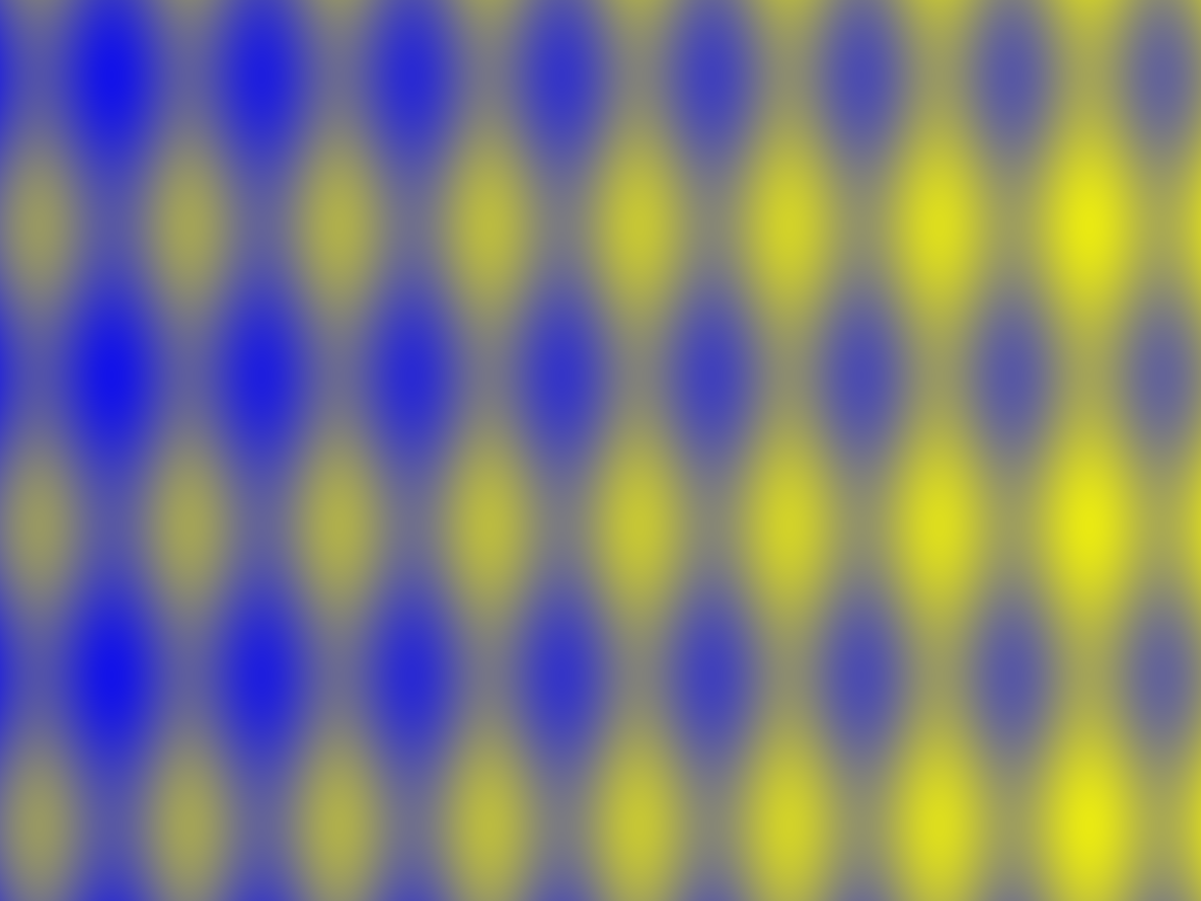
\includegraphics[width=1.1in]{images/Blue2YellowLfSensitivity} \\

    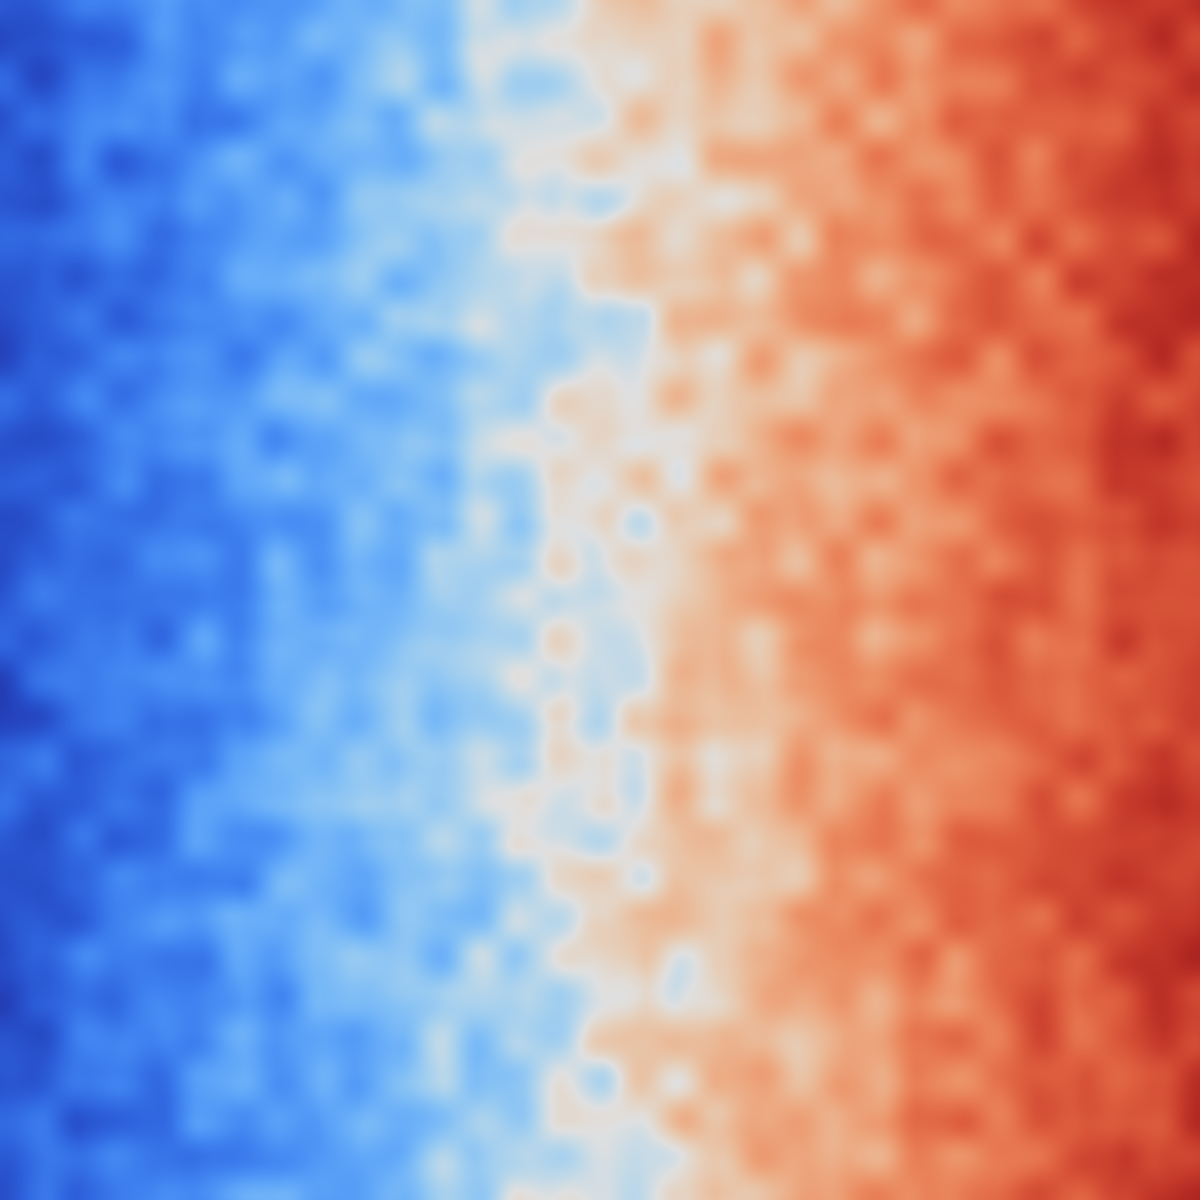
\includegraphics[width=1.1in]{images/Cool2WarmHfNoise} &
    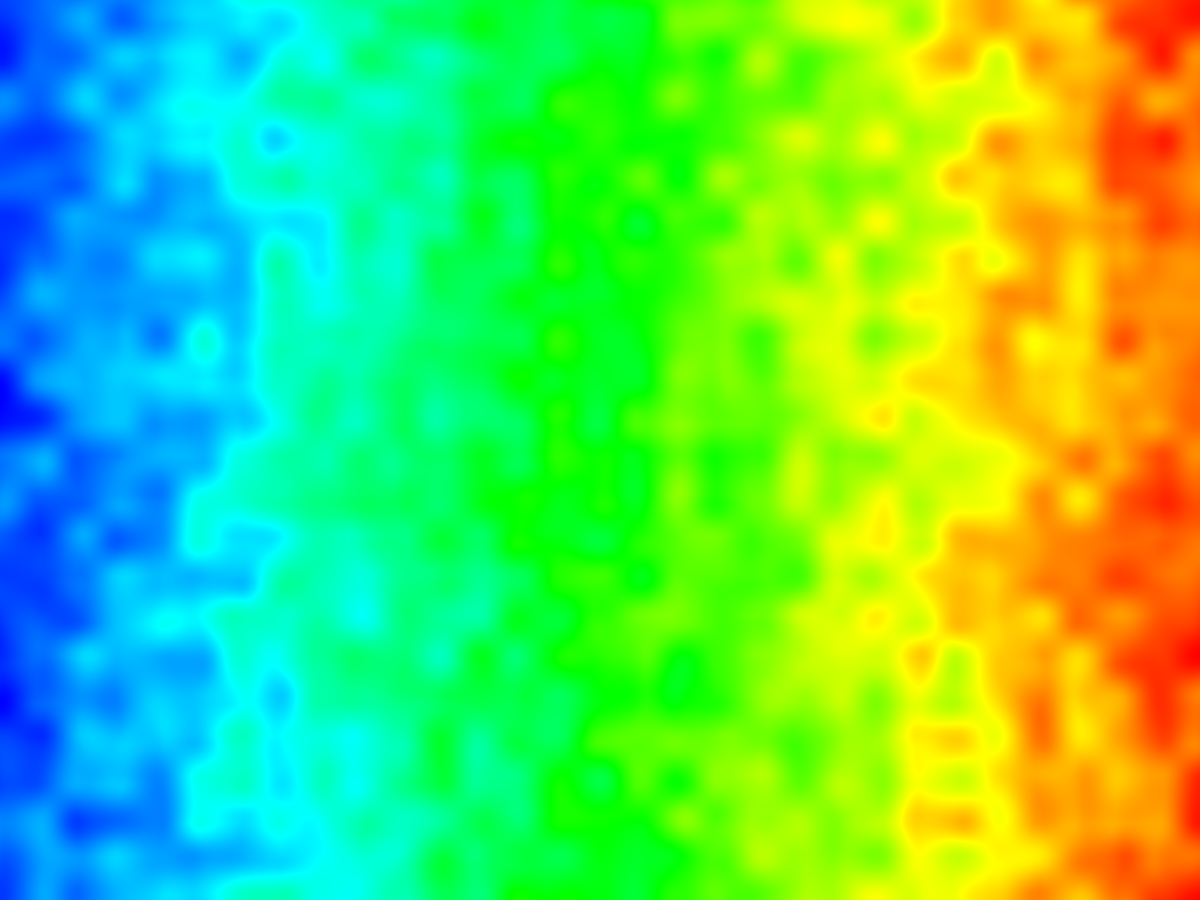
\includegraphics[width=1.1in]{images/RainbowHfNoise} &
    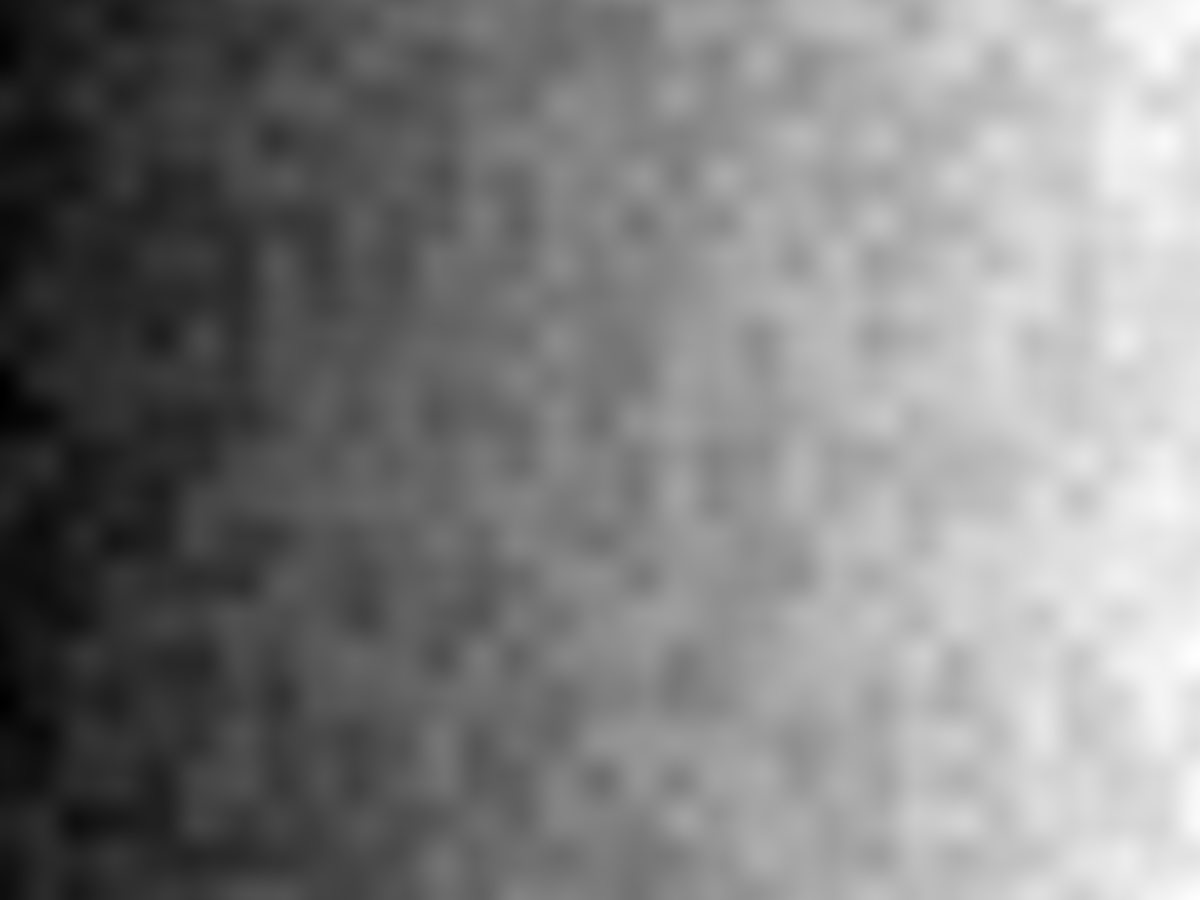
\includegraphics[width=1.1in]{images/GrayscaleHfNoise} &
    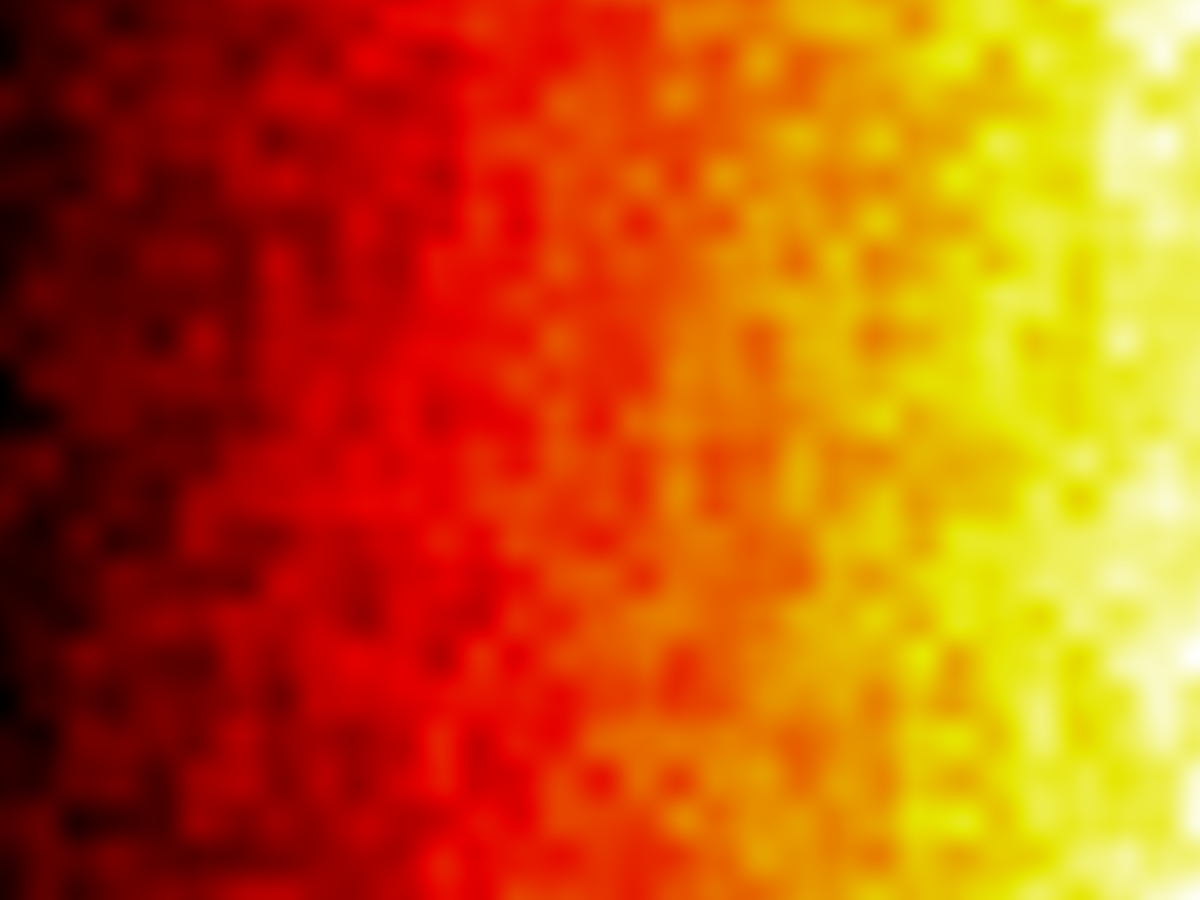
\includegraphics[width=1.1in]{images/BlackBodyHfNoise} &
    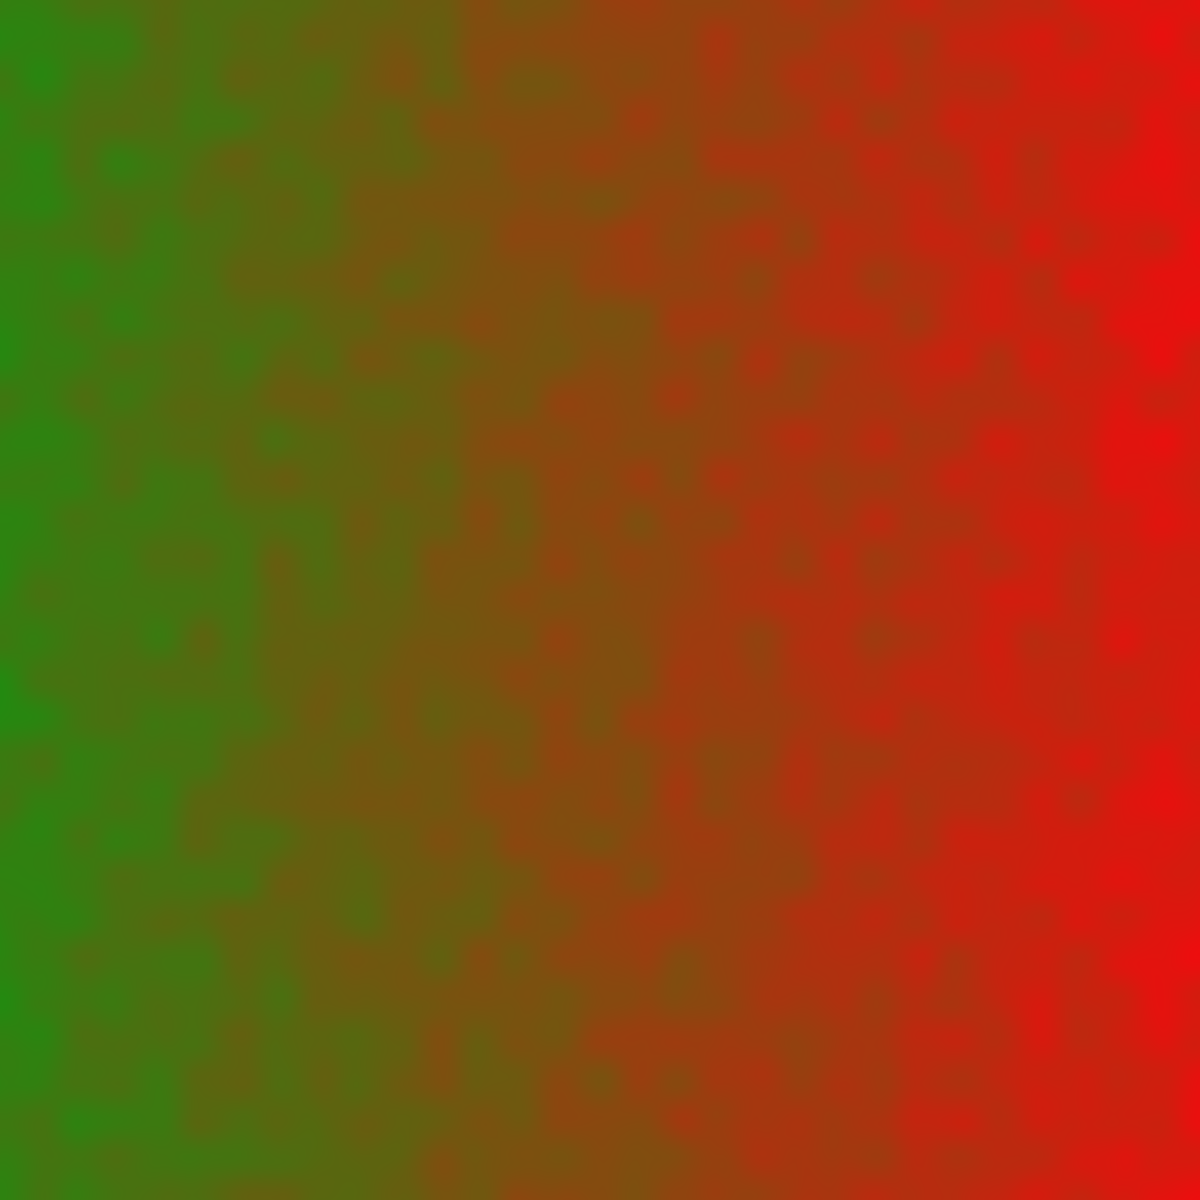
\includegraphics[width=1.1in]{images/Green2RedHfNoise} &
    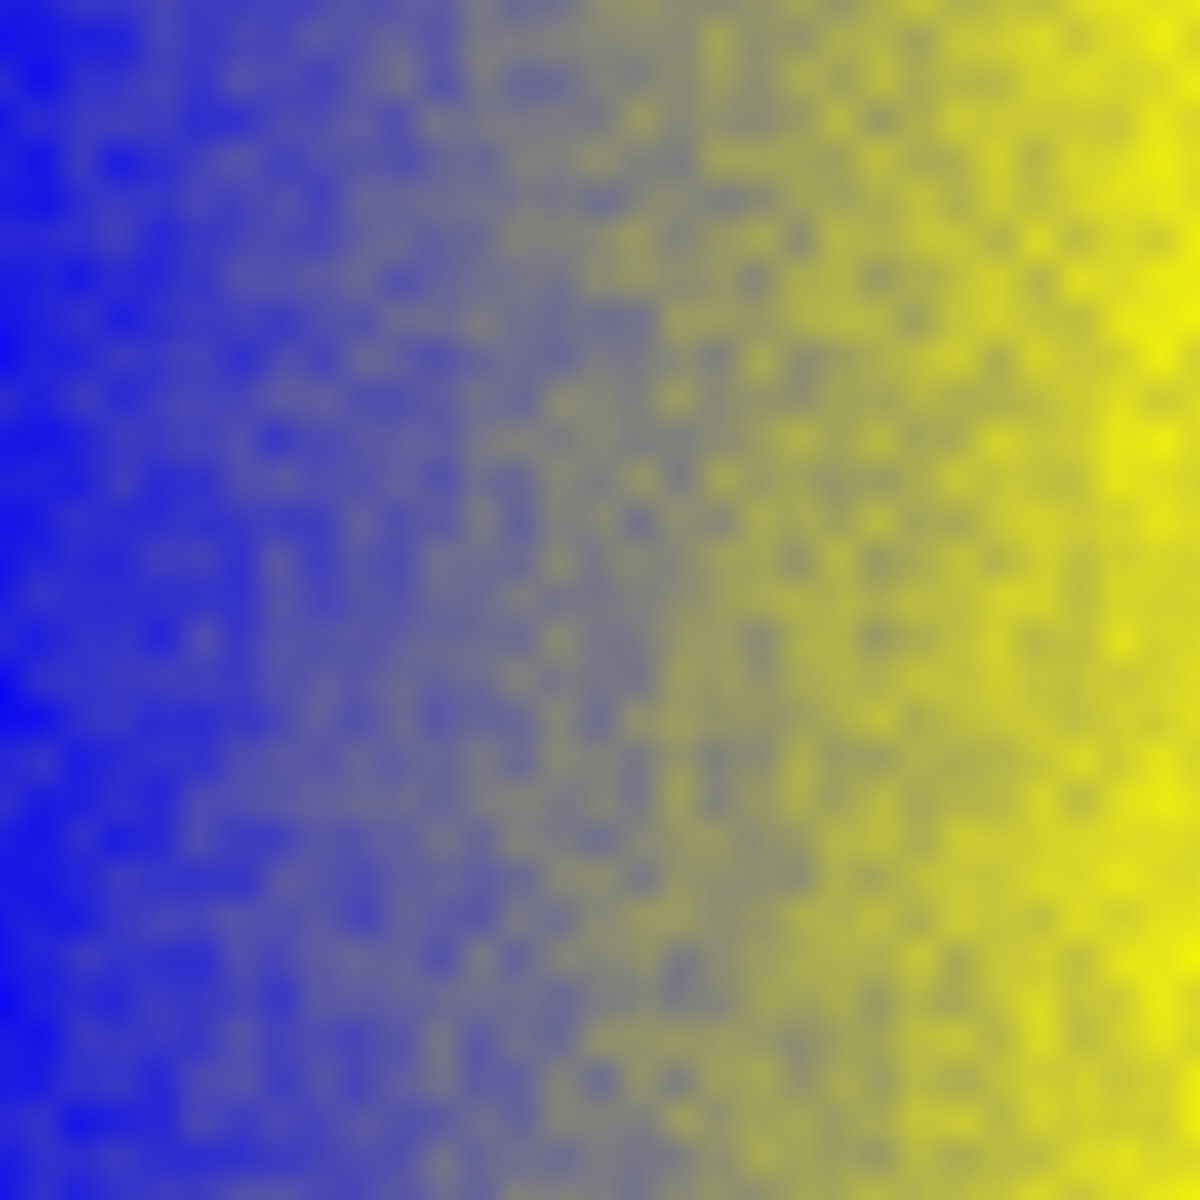
\includegraphics[width=1.1in]{images/Blue2YellowHfNoise} \\

    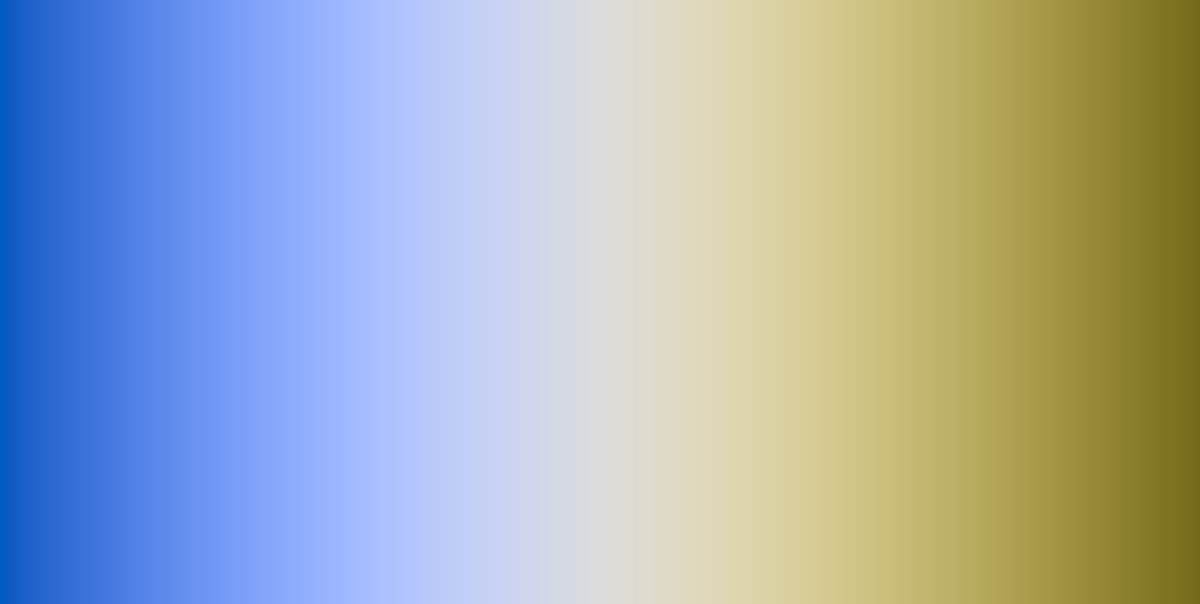
\includegraphics[width=1.1in]{images/Cool2WarmDeuteranope} &
    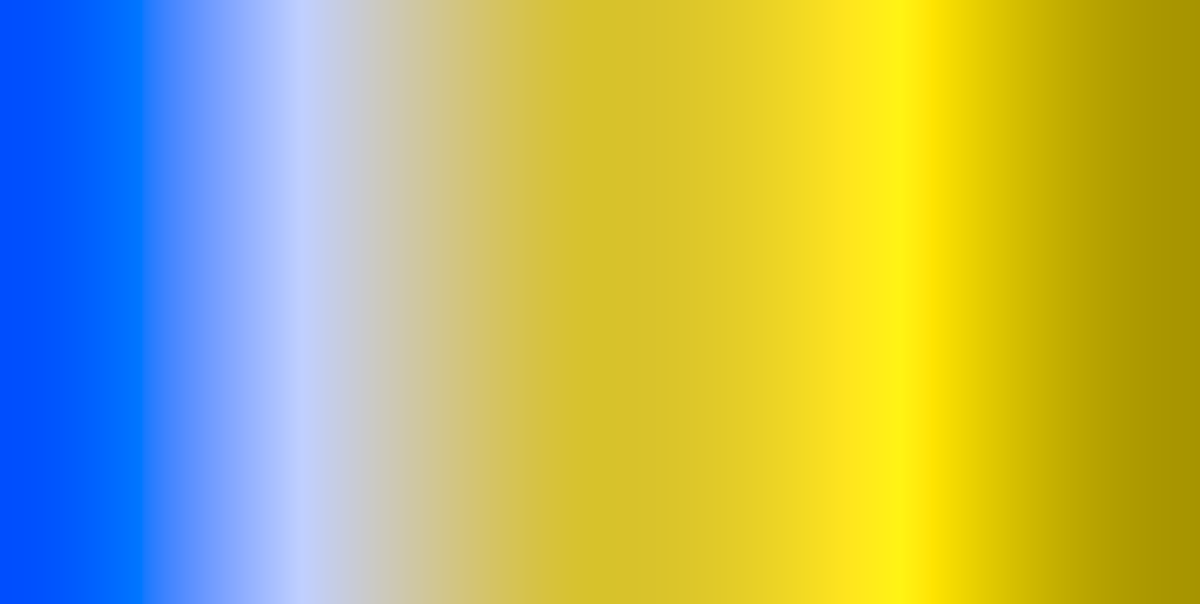
\includegraphics[width=1.1in]{images/RainbowDeuteranope} &
    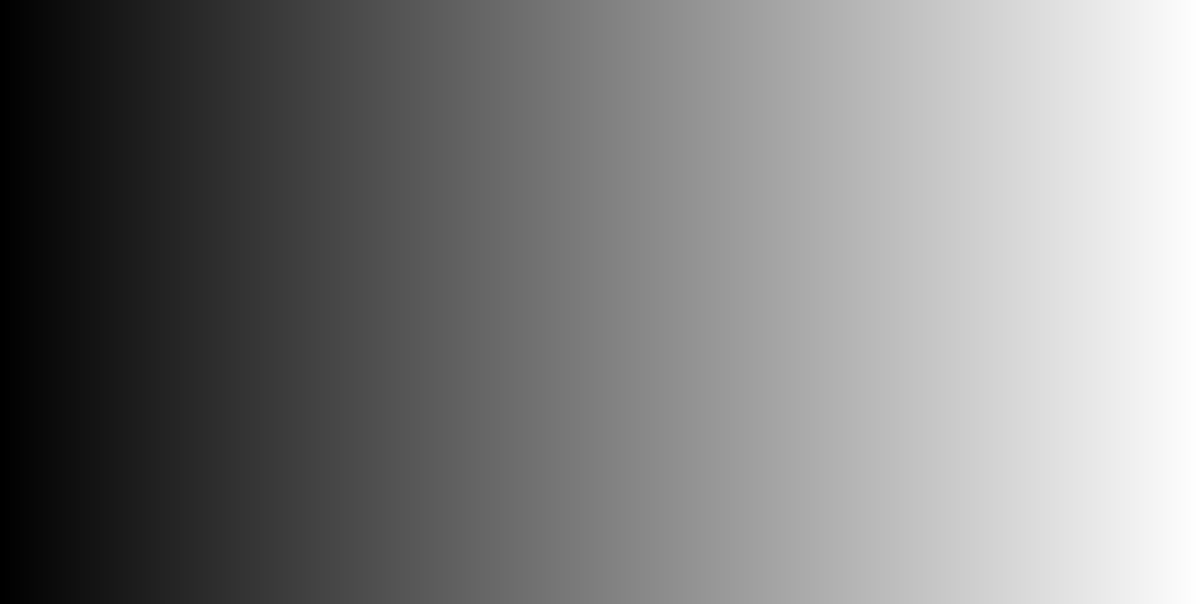
\includegraphics[width=1.1in]{images/GrayscaleDeuteranope} &
    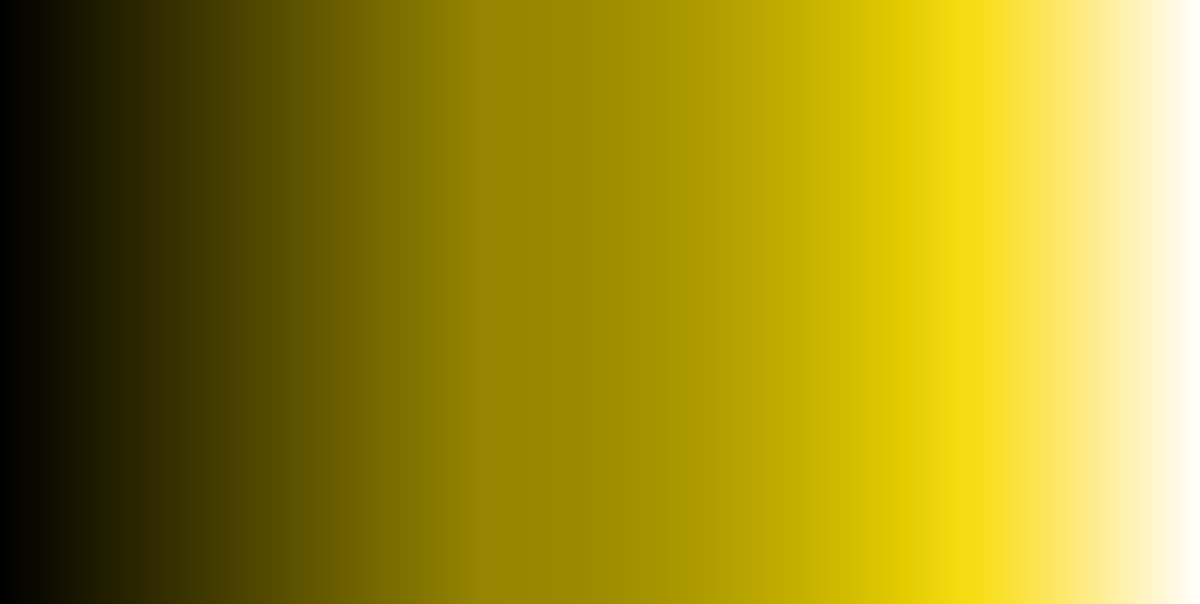
\includegraphics[width=1.1in]{images/BlackBodyDeuteranope} &
    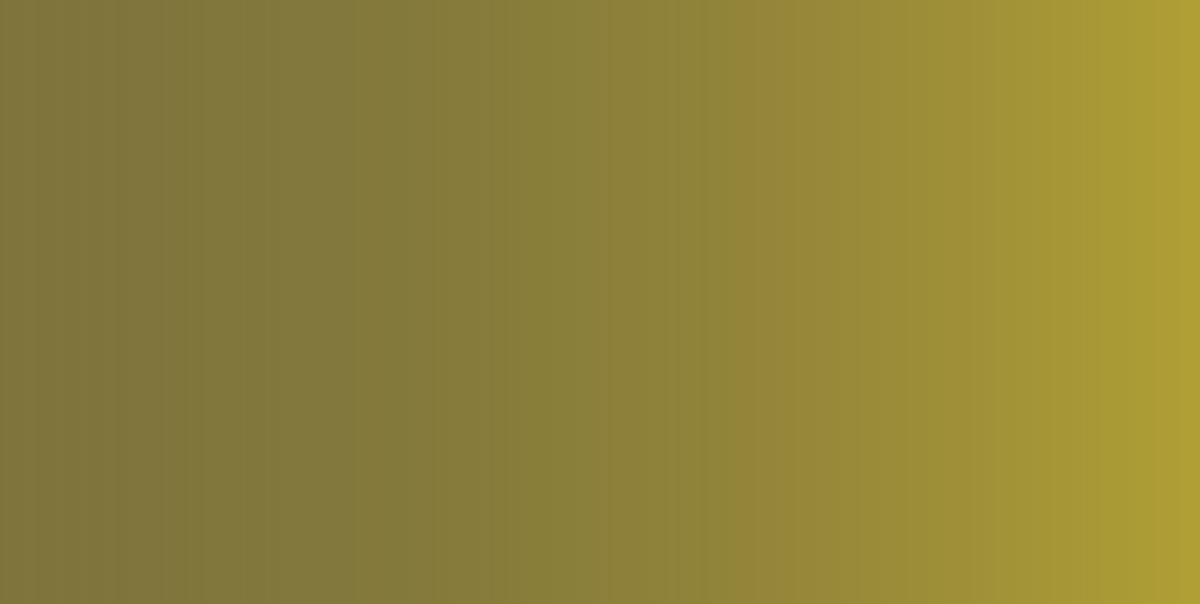
\includegraphics[width=1.1in]{images/Green2RedDeuteranope} &
    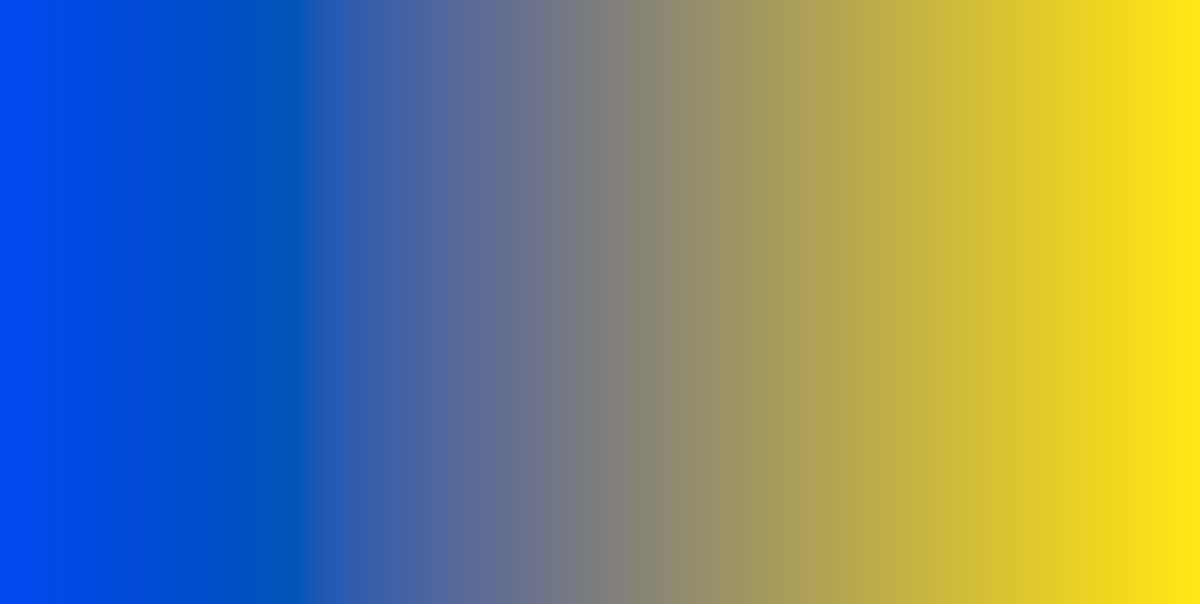
\includegraphics[width=1.1in]{images/Blue2YellowDeuteranope} \\

    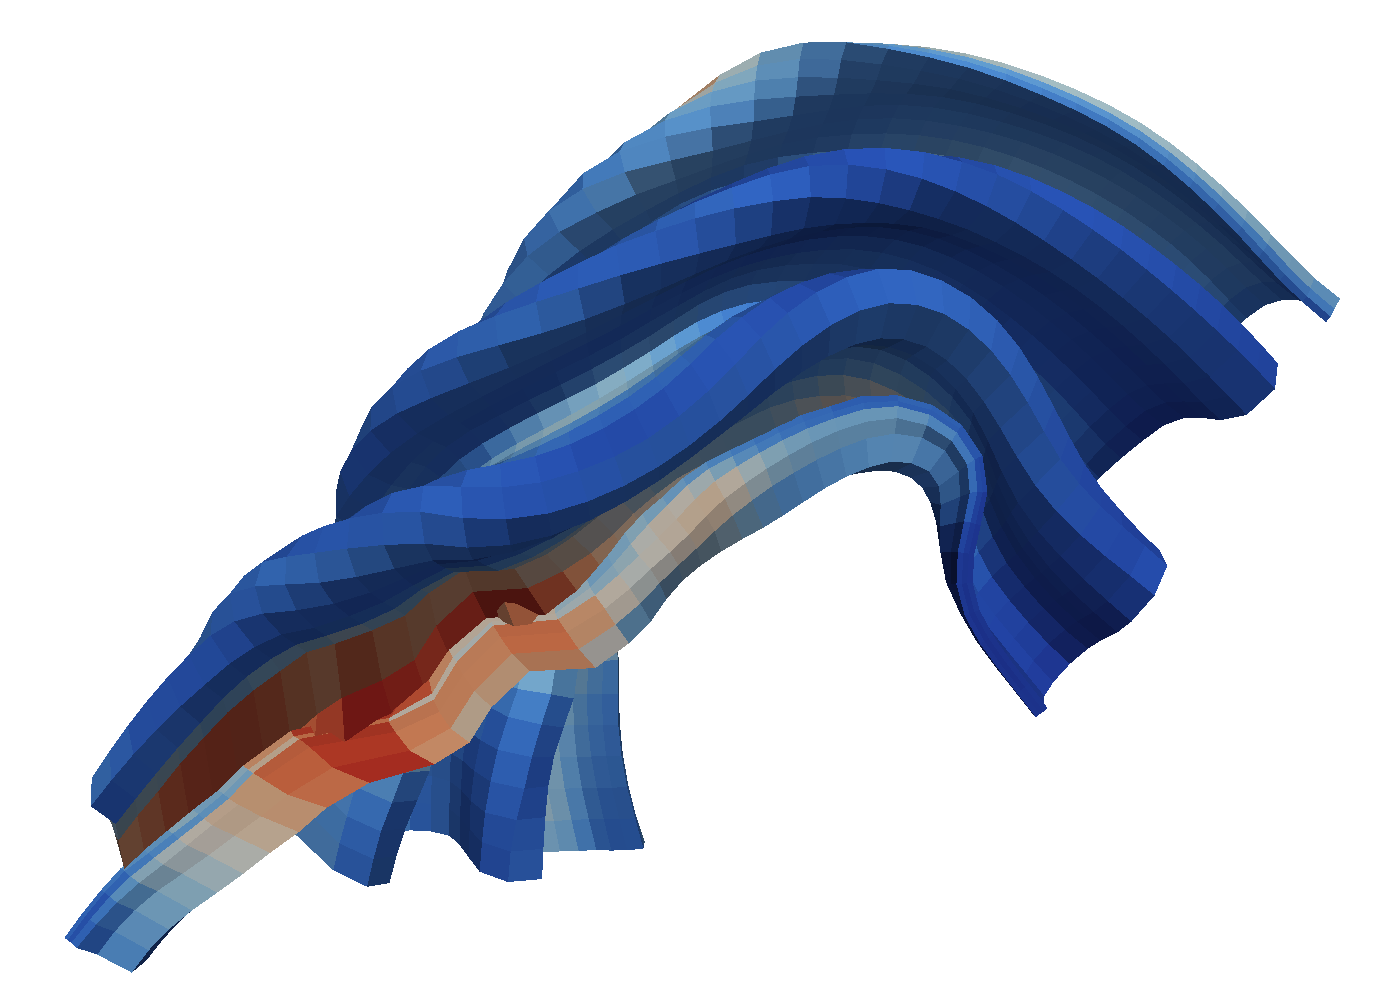
\includegraphics[width=1.1in]{images/Cool2WarmShading} &
    \includegraphics[width=1.1in]{images/RainbowShading} &
    \includegraphics[width=1.1in]{images/GrayscaleShading} &
    \includegraphics[width=1.1in]{images/BlackBodyShading} &
    \includegraphics[width=1.1in]{images/Green2RedShading} &
    \includegraphics[width=1.1in]{images/Blue2YellowShading}
  \end{tabular}
  \caption{Comparison of color map effectiveness.  The color maps are, from
    left to right, cool-warm, rainbow, grayscale, heated body, isoluminant,
    and blue-yellow.  The demonstrations are, from top to bottom, a spatial
    contrast sensitivity function, a low-frequency sensitivity function,
    high-frequency noise, an approximation of the color map viewed by
    someone with deuteranope color-deficient vision (computed with
    Vischeck), and 3D shading.}
  \label{fig:MapComparison}
\end{figure*}

Applying the design described in Section~\ref{sec:ColorMapDesign}, we can
build the cool to warm color map shown in Figure~\ref{fig:Cool2WarmBar}.
The control points, to be interpolated in \Msh space, are given in
Table~\ref{table:Cool2Warm}.  Table~\ref{table:Cool2WarmRGB} gives example
interpolated \RGB values for this color map.  \RGB values are computed from
\Lab values using a D65 white point.

\begin{table}
  \centering
  \caption{Cool to warm color map control points.}
  \begin{tabular}{c@{\qquad}ccc}
    Color & M & s & h \\
    \hline
    Red & 80 & 1.08 & 0.5 \\
    White & 88 & 0 & 1.061/-1.661 \\
    Blue & 80 & 1.08 & -1.1
  \end{tabular}
  \label{table:Cool2Warm}
\end{table}

\begin{table}
  \centering
  \caption{Cool to warm color map \RGB values.}
  \begin{tabular}{r@{.}l@{\qquad}rrr}
    \multicolumn{2}{c}{Scalar\qquad\qquad}
    		&	Red	&	Green	&	Blue	\\
    \hline
    0&0		&	59	&	76	&	192	\\
    0&03125	&	68	&	90	&	204	\\
    0&0625	&	77	&	104	&	215	\\
    0&09375	&	87	&	117	&	225	\\
    0&125	&	98	&	130	&	234	\\
    0&15625	&	108	&	142	&	241	\\
    0&1875	&	119	&	154	&	247	\\
    0&21875	&	130	&	165	&	251	\\
    0&25	&	141	&	176	&	254	\\
    0&28125	&	152	&	185	&	255	\\
    0&3125	&	163	&	194	&	255	\\
    0&34375	&	174	&	201	&	253	\\
    0&375	&	184	&	208	&	249	\\
    0&40625	&	194	&	213	&	244	\\
    0&4375	&	204	&	217	&	238	\\
    0&46875	&	213	&	219	&	230	\\
    0&5		&	221	&	221	&	221	\\
    0&53125	&	229	&	216	&	209	\\
    0&5625	&	236	&	211	&	197	\\
    0&59375	&	241	&	204	&	185	\\
    0&625	&	245	&	196	&	173	\\
    0&65625	&	247	&	187	&	160	\\
    0&6875	&	247	&	177	&	148	\\
    0&71875	&	247	&	166	&	135	\\
    0&75	&	244	&	154	&	123	\\
    0&78125	&	241	&	141	&	111	\\
    0&8125	&	236	&	127	&	99	\\
    0&84375	&	229	&	112	&	88	\\
    0&875	&	222	&	96	&	77	\\
    0&90625	&	213	&	80	&	66	\\
    0&9375	&	203	&	62	&	56	\\
    0&96875	&	192	&	40	&	47	\\
    1&0		&	180	&	4	&	38
  \end{tabular}
  \label{table:Cool2WarmRGB}
\end{table}

This diverging color map works admirably for all of our
requirements outlined in
Section~\ref{sec:ColorMapRequirements}.  The colors are aesthetically
pleasing, the order of the colors is natural, the rate of change is
perceptually linear, and the colors are still easily distinguished by those
with dichromatic vision.  The map also has a good perceptual range and
minimally interferes with shading.

Figure~\ref{fig:MapComparison} compares the cool-warm color map to some
common alternatives as well as some recommended by
Rheingans\scite{Rheingans99} and Ware\scite{Ware04}.  The cool-warm color
map works well in all the cases demonstrated here.  The rainbow color map
exhibits problems with irregular perception and sensitivity to color
deficiencies.  The grayscale and heated-body color maps work poorly in
conjunction with 3D shaded surfaces.  The isoluminant color map has a low
dynamic range and performs particularly poorly with high frequency data.
The common choice of greed-red isoluminant color maps is also useless to
most people with color-deficient vision.  The blue-yellow map works
reasonably well in all these cases, but has a lower resolution than the
cool-warm map, which yields poorer results with low contrast.

%% , as demonstrated in Figure~\ref{fig:Cool2WarmResponse}.
%% Using our initial criteria, we can think of a diverging color map as
%% ``locally'' optimal.  We cannot add or modify any color anywhere in the map
%% without degrading one or more of the requirements.

%% \begin{figure}
%%   \centering
%%   \includegraphics[height=1in]{images/Cool2WarmSpatialContrast}
%%   \quad
%%   \includegraphics[height=1in]{images/Cool2WarmShading}
%%   \caption{The spatial contrast response (left) and effect on shading
%%     (right) of the diverging color map.}
%%   \label{fig:Cool2WarmResponse}
%% \end{figure}

In addition, despite having a relatively large perceptual response, the
color map still allows for a significant amount of annotation or visual
components to be added, as shown in Figures
\ref{fig:ColorMapWithAnnotation} and \ref{fig:ColorMapOnShuttle}.

\begin{figure}
  \centering
  \includegraphics[width=\linewidth]{images/AnnotationExample}
  \caption{A terrain with the color map applied can still be annotated in
    multiple different ways. \sticky{Update with new colors.}}
  \label{fig:ColorMapWithAnnotation}
\end{figure}

\begin{figure}
  \centering
  \includegraphics[width=\linewidth]{images/ShuttleExample}
  \caption{Shuttle body with color map applied coupled with annotation and
    streamlines. \sticky{Update with new colors.}}
  \label{fig:ColorMapOnShuttle}
\end{figure}

Using the techniques described in Section~\ref{sec:ColorMapDesign}, we can
also design continuous diverging color maps with different colors.  Such
color maps may be useful in domain-specific situations when colors have
specific meaning.  Some examples are given in
Figure~\ref{fig:OtherColorMaps}.

\begin{figure}
  \centering
  \begin{tabular}{c}
    \includegraphics[width=2.5in]{images/Purple2OrangeBar} \\
    \includegraphics[width=2.5in]{images/Green2PurpleBar} \\
    \includegraphics[width=2.5in]{images/Blue2TanBar} \\
    \includegraphics[width=2.5in]{images/Green2RedDivBar}
  \end{tabular}
  \caption{Further examples of color maps defined in \Msh space.}
  \label{fig:OtherColorMaps}
\end{figure}

\sticky{A paragraph on distribution has been removed for anonymous review.}
%% An implementation of the \proc{InterpolateColor} algorithm in
%% Figure~\ref{fig:InterpolateColor} has been added to the
%% \texttt{vtkColorTransferFunction} class in the Visualization Toolkit (VTK),
%% a free, open-source scientific visualization
%% library.\footnote{\href{http://www.vtk.org}{www.vtk.org}} This diverging
%% color map interpolation has also been added to ParaView, a free, open-source
%% end-user scientific visualization
%% application.\footnote{\href{http://www.paraview.org}{www.paraview.org}}
%% Any developers or users of scientific visualization software are encouraged
%% to use these color map building tools for their own needs.


\section{Discussion}
\label{sec:Discussion}

This paper provides a color map that is a good all-around performer for
scientific visualization.  The map is an effective way to communicate data
through colors.  Because its endpoints match those of the rainbow
color map most often currently used, it can be used as a drop-in
replacement.

Diverging color maps have not traditionally been considered for most
scientific computing due to their design of a ``central'' point, which was
originally intended to have some significance.  However, with the addition
of the \Msh color space, the central point becomes a smooth neutral color
between two other colors.  The middle point serves as much to highlight the
two extremes as it does to highlight itself.  In effect, the divergent
color map allows us to quickly identify whether values are near extrema and
which extrema they are near.

This paper also provides an algorithm to generate new continuous diverging
color maps.  This interaction is useful for applying colors with domain
specific meaning or for modifying the scaling of the colors.

Although we have not been able to do user studies, the design of this color
map is based on well established theories on color perception.  This map is
a clear improvement over what is commonly used today, and I hope that many
will follow in adopting it as the new standard.


\acknowledgements{
Thanks to Russell M. Taylor II for his help on color space and color map
design.  Thanks to Patricia Crossno, Brian Wylie, Timothy Shead, and the
ParaView development team for their critical comments and general
willingness to be guinea pigs.

This work was done at Sandia National Laboratories.  Sandia is a
multiprogram laboratory operated by Sandia Corporation, a Lockheed Martin
Company, for the United States Department of Energy's National Nuclear
Security Administration under contract DE-AC04-94AL85000.
}


\bibliographystyle{abbrv}
\bibliography{ColorMaps}

\end{document}
